%\documentclass[12pt]{article}

\questionheader{ex:s3.5}


%%%%%%%%%%%%%%%%%%
\subsection*{\Conceptual}
%%%%%%%%%%%%%%%%%%

%%%%%%%%%%%%%%%%%%%%%%%%%%%%%%%%
\begin{question}
Evaluate the integral 
\begin{equation*}
\text{$\dblInt_R \sqrt{b^2-y^2}\ \dee{x}\,\dee{y}$\ \  
where $R$ is the rectangle  $0\le x\le a,\ 0\le y\le b$}
\end{equation*}
\emph{without} using iteration. Instead, interpret the integral 
geometrically.
\end{question}

%\begin{hint}
%
%\end{hint}

\begin{answer}
$\frac{1}{4}\pi ab^2$
\end{answer}

\begin{solution}
$\dblInt_R \sqrt{b^2-y^2}\,\dee{x}\,\dee{y}
=\tripInt_V \dee{x}\,\dee{y}\,\dee{z}$, where 
\begin{align*}
V&=\Set{(x,y,z)} {0\le z\le\sqrt{b^2-y^2},\  0\le x\le a,\  0\le y\le b} \\
 &=\Set{(x,y,z)} {y^2+z^2\le b^2,\  0\le x\le a,\  y\ge 0,\ z\ge 0}
\end{align*}
Now $y^2+z^2\le b^2$ is a cylinder of radius $b$ centered on the $x$--axis and the part of $y^2+z^2\le b^2$, with $y\ge0,\ z\ge0$ is one quarter of this cylinder.
It has cross--sectional area $\frac{1}{4}\pi b^2$. $V$ is the part of
this quarter--cylinder with $0\le x\le a$. It has length $a$ and 
cross--sectional area $\frac{1}{4}\pi b^2$. So, 
$\dblInt_R \sqrt{b^2-y^2}\,\dee{x}\,\dee{y}=\frac{1}{4}\pi ab^2$.
\end{solution}


\begin{question}[M200 2013D] %1g
Find the total mass of the rectangular box 
$[0, 1] \times [0, 2] \times [0, 3]$ (that is, the box
defined by the inequalities $0 \le x \le 1$, $0 \le y \le 2$, 
$0 \le z \le 3$), with density function $h(x, y, z) = x$.
\end{question}

%\begin{hint}
%
%\end{hint}

\begin{answer}
$3$
\end{answer}

\begin{solution}
The mass is
\begin{align*}
\int_0^1\dee{x} \int_0^2\dee{y}\int_0^3\dee{z}\ x
&= 6\int_0^1 \dee{x}\ x =3
\end{align*}
\end{solution}

%%%%%%%%%%%%%%%%%%%%%%%%%%%%
%\Instructions{Questions~\ref{prob_s1.0first} through \ref{prob_s1.0last} provide practice with.}
%%%%%%%%%%%%%%%%%%%%

%%%%%%%%%%%%%%%%%%
\subsection*{\Procedural}
%%%%%%%%%%%%%%%%%%

%%%%%%%%%%%%%%%%%%%%%%%%%%%%%%%%
\begin{question}
Evaluate $\dst\tripInt_R x\ \dee{V}$ where $R$ is the tetrahedron bounded
by the coordinate planes and the plane 
$\frac{x}{a}+\frac{y}{b}+\frac{z}{c}=1$.
\end{question}

%\begin{hint}
%
%\end{hint}

\begin{answer}
$\frac{a^2bc}{24}$
\end{answer}

\begin{solution}
The domain of integration is  
\begin{equation*}
V=\Set{(x,y,z)}{x,y,z\ge 0,\ \tfrac{x}{a}+\tfrac{y}{b}+\tfrac{z}{c}\le 1}
\end{equation*}
\begin{itemize}
\item
In $V$, $\tfrac{z}{c}\le 1-\tfrac{x}{a}-\tfrac{y}{b}$ and $x,y\ge0$, so
the biggest value of $z$ in $V$ is achieved when $x=y=0$ and is $c$. 
Thus, in $V$, $z$ runs from $0$ to $c$.
\item
For each fixed $0\le z\le c$, $(x,y)$ takes all values in
\begin{equation*}
D_z=\Set{(x,y)}{x,y\ge 0,\ \tfrac{x}{a}+\tfrac{y}{b}\le 1-\tfrac{z}{c}}
\end{equation*}
The biggest value of $y$ on $D_z$ is achieved when $x=0$ and is $b\left(1-\tfrac{z}{c}\right)$. Thus, on $D_z$, $y$ runs from $0$ to 
$b\left(1-\tfrac{z}{c}\right)$.
\item
For each fixed $0\le z\le c$ and
 $0\le y \le b\left(1-\tfrac{z}{c}\right)$, $x$ runs over
\begin{equation*}
D_{y,z}=\Set{x}{0\le x \le a\left(1-\tfrac{y}{b}-\tfrac{z}{c}\right)}
\end{equation*}
This is pictured in the figure on the right below.
\end{itemize}

\begin{center}
     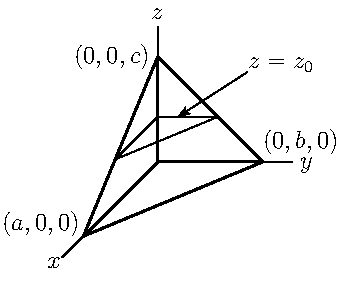
\includegraphics{domainTetrahedron.pdf}\qquad
     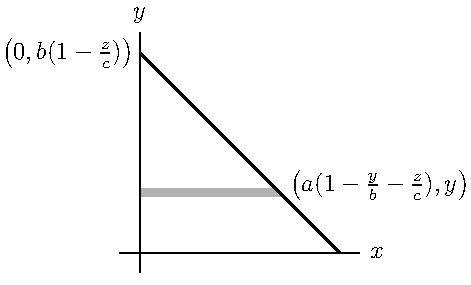
\includegraphics{domainTetrahedron2.pdf}
\end{center} 

So the specified integral is
\begin{align*}
\tripInt_R x\ \dee{V}
&=\int_0^c \dee{z} \dblInt_{D_z} \dee{x}\,\dee{y}\ x
 = \int_0^c \dee{z}\int_0^{b(1-{z\over c})}\dee{y}\int_{D_{y,z}}\dee{x}\ x\\
&=\int_0^c \dee{z}\int_0^{b(1-{z\over c})}\dee{y}
             \int_0^{a(1-{y\over b}-{z\over c})} \dee{x}\ x
=\int_0^c \dee{z}\int_0^{b(1-{z\over c})} \dee{y}\ \frac{a^2}{2}
\left(1-\frac{y}{b}-\frac{z}{c}\right)^2 \\
&=\int_0^c \dee{z}\ \left[-\frac{a^2b}{6}
           \left(1-\frac{y}{b}-\frac{z}{c}\right)^3
                                    \right]_0^{b(1-{z\over c})}
=\int_0^c \dee{z}\ \frac{a^2b}{6}\left(1-\frac{z}{c}\right)^3 \\
&=\left[-\frac{a^2bc}{24}\left(1-\frac{z}{c}\right)^4  \right]_0^c
=\frac{a^2bc}{24}
\end{align*}
\end{solution}

%%%%%%%%%%%%%%%%%%%%%%%%%%%%%%%%
\begin{question}
Evaluate $\dst\tripInt_R y\ \dee{V}$ where $R$ is the portion
of the cube $0\le x,y,z\le 1$ lying above the plane $y+z=1$ and below the 
plane $x+y+z=2$.
\end{question}

%\begin{hint}
%
%\end{hint}

\begin{answer}
$\frac{5}{24}$
\end{answer}

\begin{solution}
The domain of integration is 
\begin{equation*}
R = \Set{(x,y,z)}{0\le x,y,z\le 1,\ z\ge 1-y,\ z\le2-x-y}
\end{equation*}
In the figure on the  below, the more darkly shaded region 
is part of $z=1-y$ and the more lightly shaded region is part
of $z=2-x-y$. 
\begin{center}
     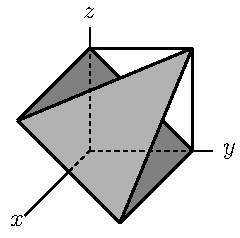
\includegraphics{domainPartCube1.pdf}
\end{center} 
\begin{itemize}
\item
In $R$, $z$ runs from $0$ (for example $(0,1,0)$ is in $R$)
to $1$ (for example $(0,0,1)$ is in $R$).
\item
For each fixed $0\le z\le 1$, $(x,y)$ runs over
\begin{equation*}
D_z = \Set{(x,y)}{0\le x,y\le 1,\ y\ge 1-z,\ x+y\le2-z}
\end{equation*}
Here is a sketch of a top view of $D_z$.
\begin{center}
     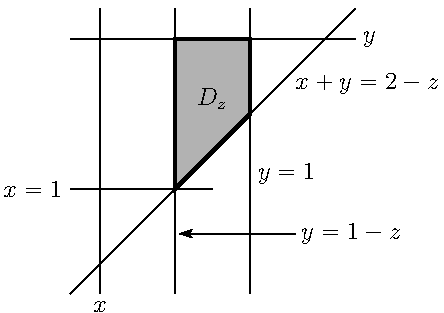
\includegraphics{domainPartCube2.pdf}
\end{center} 
On $D_z$, $y$ runs from $1-z$ to $1$.
\item
For each fixed $0\le z\le 1$ and $1-z\le y\le 1$, $x$ runs from $0$
to $2-y-z$. 
\end{itemize}
So the specified integral is
\begin{align*}
\tripInt_R y\ \dee{V}
&=\int_0^1\dee{z}\dblInt_{D_z} \dee{x}\dee{y}\ y
=\int_0^1 \dee{z}\int_{1-z}^1 \dee{y}\int_0^{2-y-z} \dee{x}\ y
=\int_0^1 \dee{z}\int_{1-z}^1 \dee{y}\ y(2-y-z)\cr
&=-\int_0^1 \dee{z}\int_z^0 du\ (1-u)(1+u-z)\qquad\text{ where $u=1-y$}\\
&=\int_0^1 \dee{z}\int_0^z du\ (1-u^2-z+uz)
=\int_0^1 \dee{z}\ \big(z-\frac{z^3}{3}-z^2+\frac{z^3}{2})\\
&=\frac{1}{2}-\frac{1}{12}-\frac{1}{3}+\frac{1}{8}
=\frac{5}{24}
\end{align*}
\end{solution}

%%%%%%%%%%%%%%%%%%%%%%%%%%%%%%%%
\begin{question}
For each of the following, express the given iterated integral as an
iterated integral in which the integrations are  performed in the order:
first $z$, then $y$, then $x$.
\begin{enumerate}[(a)]
\item
$\dst\int_0^1\dee{z}\int_0^{1-z}\dee{y}\int_0^{1-z} \dee{x}\ f(x,y,z)$
\item
$\dst\int_0^1\dee{z}\int_{\sqrt z}^1\dee{y}\int_0^y \dee{x}\ f(x,y,z)$
\end{enumerate}
\end{question}

%\begin{hint}
%
%\end{hint}

\begin{answer}
(a) $\dst\int_0^1\dee{x}\int_0^{x}\dee{y}\int_0^{1-x}\hskip-10pt \dee{z}\hskip3pt f(x,y,z)
+\int_0^1\dee{x}\int_x^{1}\dee{y}\int_0^{1-y}\hskip-10pt \dee{z}\hskip3pt f(x,y,z)$

(b) $\dst\int_0^1\dee{x}\int_x^{1}\dee{y}\int_0^{y^2}\!\! \dee{z}\  f(x,y,z)$
\end{answer}

\begin{solution}
(a)
 The domain of integration is 
\begin{align*}
V &= \Set{(x,y,z)}{0\le z\le 1,\ 0\le y\le 1-z,\ 0\le x\le 1-z} \\
  &= \Set{(x,y,z)}{ x,y,z\ge 0,\ x+z\le 1,\ y+z\le 1 }
\end{align*}
This is sketched in the figure below. The front face is $x+z=1$ and the 
lightly shaded right face is $y+z=1$.
\begin{center}
     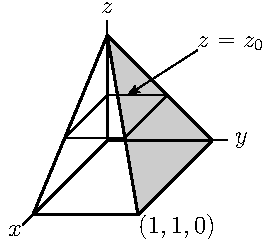
\includegraphics{domainFivehedron1.pdf}
\end{center}
In $V$, 
\begin{itemize}
\item
$x$ takes all values between $0$ and $1$. 
\item
For each fixed $0\le x\le 1$, $(y,z)$ takes all values in
\begin{equation*}
D_x=\Set{(y,z)}{y,z\ge 0,\ z\le 1-x,\ y+z\le 1}
\end{equation*}
Here is a sketch of $D_x$.
\begin{center}
     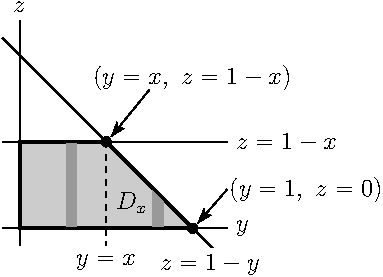
\includegraphics{domainFivehedron2.pdf}
\end{center}
\item 
Looking at the sketch above, we see that, on $D_x$, $y$ runs from $0$ to $1$
and
\begin{itemize}
\item
for each fixed $y$ between $0$ and $x$, $z$ runs from $0$ to $1-x$ and
\item
for each fixed $y$ between $x$ and $1$, $z$ runs from $0$ to $1-y$
\end{itemize}
\end{itemize}
So the integral is, in the new order, 
\begin{align*}
\tripInt_V f(x,y,z)\ \dee{V}
&= \int_0^1\dee{x}\dblInt_{D_x} \dee{y}\,\dee{z}\ f(x,y,z) \\
&= \int_0^1\dee{x}\int_0^{x}\dee{y}\int_0^{1-x}\hskip-10pt \dee{z}\hskip3pt f(x,y,z)
+\int_0^1\dee{x}\int_x^{1}\dee{y}\int_0^{1-y}\hskip-10pt \dee{z}\hskip3pt f(x,y,z)
\end{align*}


(b) The domain of integration is 
\begin{align*}
V &= \Set{(x,y,z)}{0\le z\le 1,\ \sqrt{z}\le y\le 1,\ 0\le x\le y} \\
  &= \Set{(x,y,z)}{0\le z\le y^2,\ 0\le x\le y\le 1} 
\end{align*}
In this region, $x$ takes all values between $0$ and $1$. For each fixed
$x$ between $0$ and $1$, $(y,z)$ takes all values in
\begin{equation*}
D_x=\Set{(y,z)}{0\le z\le y^2,\ x\le y\le 1}
\end{equation*}
Here is a sketch of $D_x$.
\begin{center}
     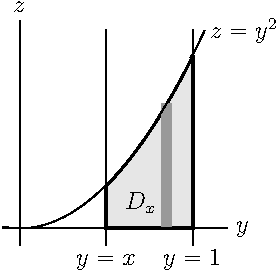
\includegraphics{domainSwitchb.pdf}
\end{center}
In the new order, the integral is
\begin{equation*}
\int_0^1\dee{x}\dblInt_{D_x} \dee{y}\,\dee{z}\ f(x,y,z)
=\int_0^1\dee{x}\int_x^{1}\dee{y}\int_0^{y^2}\!\! \dee{z}\  f(x,y,z)
\end{equation*}
\end{solution}

%%%%%%%%%%%%%%%%%%%%%%%%%%%%%%%%
\begin{question}[M200 2005D] %9
A triple integral $\dst\tripInt_E f\ \dee{V}$ is given in 
iterated form by
\begin{equation*}
\int_{y=-1}^{y=1} \int_{z=0}^{z=1-y^2} \int_{x=0}^{2-y-z} f(x,y,z)
                                    \ \dee{x}\,\dee{z}\,\dee{y}
\end{equation*}
\begin{enumerate}[(a)]
\item
Draw a reasonably accurate picture of $E$ in 3--dimensions. Be sure 
to show the units on the coordinate axes.
\item
Rewrite the triple integral $\tripInt_E f\ \dee{V}$ as one or more 
iterated triple integrals in the order
\begin{equation*}
\int_{y=}^{y=} \int_{x=}^{x=} \int_{z=}^{z=} f(x,y,z)
                                    \ \dee{z}\,\dee{x}\,\dee{y}
\end{equation*}
\end{enumerate}
\end{question}

%\begin{hint}
%
%\end{hint}

\begin{answer}
(a)
\begin{center}
     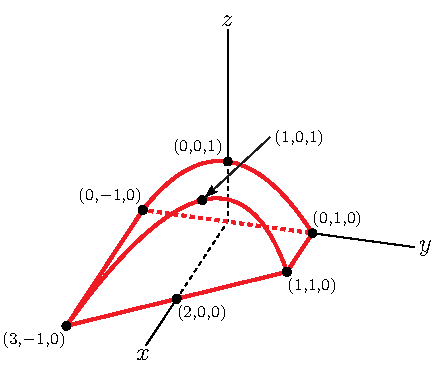
\includegraphics{OE05D_9c.pdf}
\end{center}

(b)
\begin{align*}
&\int_{y=-1}^{y=1} \int_{x=0}^{x=1+y^2-y} \int_{z=0}^{z=1-y^2} f(x,y,z)
                                    \ \dee{z}\,\dee{x}\,\dee{y} \\
&\hskip1in
+\int_{y=-1}^{y=1} \int_{x=1+y^2-y}^{x=2-y} \int_{z=0}^{z=2-x-y} f(x,y,z)
                                    \ \dee{z}\,\dee{x}\,\dee{y}
\end{align*}
\end{answer}

\begin{solution}
(a) In the domain of integration for the given integral
\begin{itemize}
\item
$y$ runs from $-1$ to $1$, and
\item
for each fixed $y$ in that range $z$ runs from $0$ to $1-y^2$, and
\item
for each fixed $y$ and $z$ as above, $x$ runs from $0$ to $2-y-z$.
\end{itemize}
That is,
\begin{equation*}
E = \Set{(x,y,z)}{-1\le y\le 1,\ 0\le z\le 1-y^2,\ 0\le x\le 2-y-z}
\end{equation*}
\begin{itemize}
\item
Each constant $x$ cross--section of the surface $z=1-y^2$ is an upside
down parabola. So the surface $z=1-y^2$ consists of a bunch of copies of the
parabola $z=1-y^2$ stacked front to back. The figure of the left below
provides a sketch of $z=1-y^2$.

\item
The surface $x = 2-y-z$, or equivalently, $x+y+z=2$ is a plane.
It passes through the points  $(2,0,0)$, $(0,2,0)$ and $(0,0,2)$.
It is sketched in the figure on the right below. We know that our
domain of integration extends to $y=-1$, so we have chosen to include
in the sketch the part of the plane in $x\ge 0$, $y\ge-1$, $z\ge 0$.

\end{itemize}
\begin{center}
     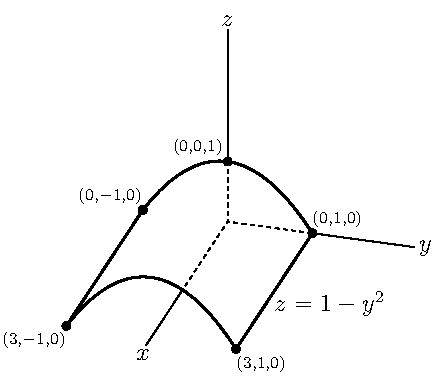
\includegraphics{OE05D_9a.pdf}\quad
     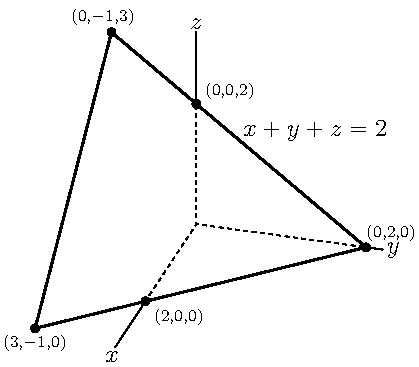
\includegraphics{OE05D_9b.pdf}
\end{center}
The domain $E$ is constructed by using the plane $x+y+z=2$
to chop the front off of the ``tunnel'' $0\le z\le 1-y^2$.
It is outlined in red in the figure below.

\begin{center}
     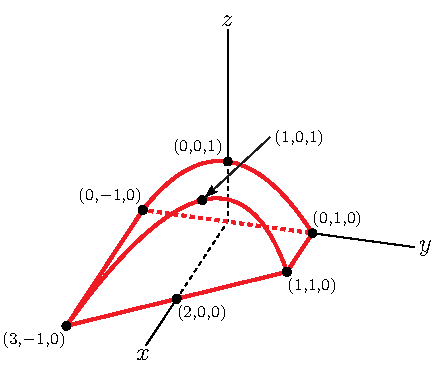
\includegraphics{OE05D_9c.pdf}
\end{center}

(b) We are to change the order of integration so that the outside 
integral is over $y$ (the same as the given integral),
the middle integral is over $x$, and the inside integral is over
over $z$. 
\begin{itemize}
\item
We still have $y$ running from $-1$ to $1$.
\item
For each fixed $y$ in that range, $(x,z)$ runs over
\begin{equation*}
E_y=\Set{(x,z)}{0\le z\le 1-y^2,\ 0\le x+z\le 2-y}
\end{equation*}
\item 
The biggest value of $x$ in $E_y$ is $2-y$. It is achieved
when $z=0$. You can also see this in the figure below.
The shaded region in that figure is $E_y$.
\item
For each fixed $x$ and $y$ as above,  $z$ runs over
\begin{equation*}
E_{x,y} = \Set{z}{0\le z\le 1-y^2,\ 0\le z\le 2-x-y}
\end{equation*}
That is, $z$ runs from $0$ to the smaller of
$1-y^2$ and $2-x-y$. Note that $1-y^2\le 2-x-y$
if and only if $x\le 1+y^2-y$.
\item
So if $0\le x\le 1+y^2-y$, $z$ runs from $0$ to $1-y^2$
and if $1+y^2-y\le x\le 2-y$, $z$ runs from $0$ to $2-x-y$.
\end{itemize}

\begin{center}
     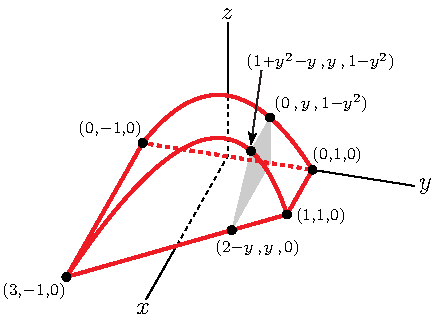
\includegraphics{OE05D_9d.pdf}
\end{center}

So the integral is
\begin{align*}
&\int_{y=-1}^{y=1} \int_{x=0}^{x=1+y^2-y} \int_{z=0}^{z=1-y^2} f(x,y,z)
                                    \ \dee{z}\,\dee{x}\,\dee{y} \\
&\hskip1in
+\int_{y=-1}^{y=1} \int_{x=1+y^2-y}^{x=2-y} \int_{z=0}^{z=2-x-y} f(x,y,z)
                                    \ \dee{z}\,\dee{x}\,\dee{y}
\end{align*}
\end{solution}


%%%%%%%%%%%%%%%%%%%%%%%%%%%%%%%%
\begin{question}[M200 2006D] %6a
A triple integral $\tripInt_E f(x,y,z)\ \dee{V}$ is given in the 
iterated form
\begin{equation*}
J = \int_0^1 \int_0^{1-\frac{x}{2}} \int_0^{4-2x-4z} f(x,y,z)
                                    \ \dee{y}\,\dee{z}\,\dee{x}
\end{equation*}
\begin{enumerate}[(a)]
\item
Sketch the domain $E$ in 3--dimensions. Be sure to show the units.
\item
Rewrite the integral as one or more iterated integrals in the form
\begin{equation*}
J = \int_{y=}^{y=} \int_{x=}^{x=} \int_{z=}^{z=} f(x,y,z)
                                    \ \dee{z}\,\dee{x}\,\dee{y}
\end{equation*}
\end{enumerate}
\end{question}

%\begin{hint}
%
%\end{hint}

\begin{answer}
(a)

\begin{center}
     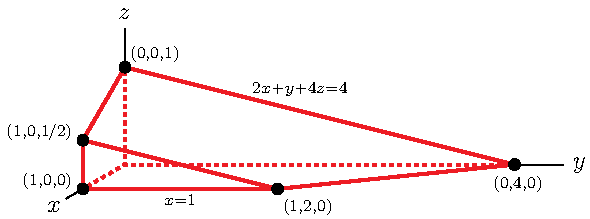
\includegraphics{OE06D_6a3.pdf}
\end{center}

(b)
\begin{align*}
J = \int_{y=0}^{y=2} \int_{x=0}^{x=1} \int_{z=0}^{z=\frac{4-2x-y}{4}}
        \!\!\!\! f(x,y,z)  \ \dee{z}\,\dee{x}\,\dee{y}
+\int_{y=2}^{y=4} \int_{x=0}^{x=\frac{4-y}{2}} \int_{z=0}^{z=\frac{4-2x-y}{4}} 
        \!\!\!\!  f(x,y,z)\ \dee{z}\,\dee{x}\,\dee{y}
\end{align*}

\end{answer}

\begin{solution}
(a) In the given integral $J$,
\begin{itemize}
\item
$x$ runs from $0$ to $1$,
\item
for each fixed $x$ in that range, $z$ runs from 0 to $1-\frac{x}{2}$, and
\item
for each fixed $x$ and $z$ as above, $y$ runs from $0$ to $4-2x-4z$.
\end{itemize}
So 
\begin{align*}
E = \Set{(x,y,z)}{0\le x\le 1,\ 0\le z\le 1-\tfrac{x}{2},\ 
            0 \le y\le 4-2x-4z}
\end{align*}
Notice that the condition $y\le 4-2x-4z$ can be rewritten
as $z\le 1-\frac{x}{2} -\frac{y}{4}$. When $y\ge 0$, this implies
that $z\le 1-\frac{x}{2}$, so that we can drop the condition 
$z\le 1-\frac{x}{2}$ from our description of $E$:
\begin{align*}
E = \Set{(x,y,z)}{0\le x\le 1,\ 0 \le y\le 4-2x-4z,\ z\ge 0}
\end{align*}



First, we figure out what $E$ looks like. 
The plane $2x+y+4z=4$ intersects the $x$--, $y$-- and $z$--axes
at $(2,0,0)$, $(0,4,0)$ and $(0,0,1)$, respectively.
That plane is shown in the sketch on the left below.
The set of points $\Set{(x,y,z)}{x,y,z\ge 0,\  y\le 4-2x-4z}$
is outlined with heavy lines.
\begin{center}
     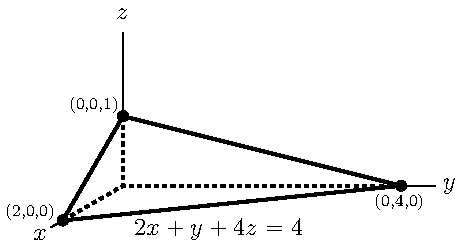
\includegraphics[scale=0.99]{OE06D_6a2.pdf}\quad
     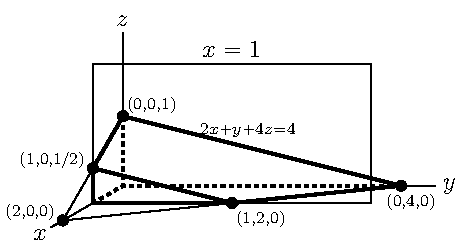
\includegraphics[scale=0.99]{OE06D_6a1.pdf}
\end{center}
So it only remains to impose the condtion $x\le 1$, which chops off
the front bit of the tetrahedron. This is done in the sketch on the
right above. Here is a cleaned up sketch of $E$.
\begin{center}
     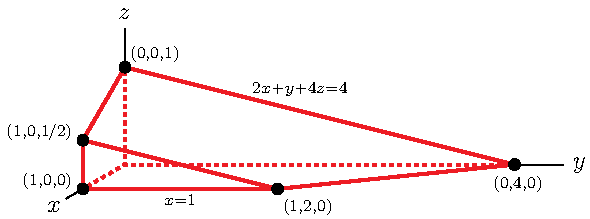
\includegraphics{OE06D_6a3.pdf}
\end{center}

(b)
We are to reorder the integration so that the outside integral
is over $y$, the middle integral is over $x$, and the inside integral 
is over $z$. Looking at the figure below, 
\begin{center}
     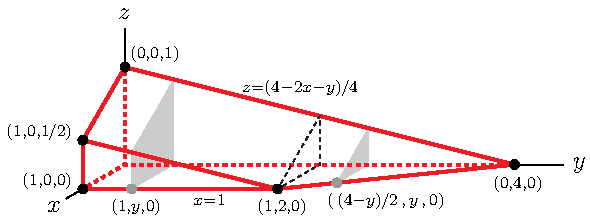
\includegraphics{OE06D_6a4.pdf}
\end{center}
we see that
\begin{itemize}
\item
$y$ runs from $0$ to $4$, and
\item
for each fixed $y$ in that range, $(x,z)$ runs over
\begin{equation*}
\Set{(x,z)}{0\le x\le 1,\ 2x+4z\le 4-y,\ z\ge 0}
\end{equation*}
\item
for each fixed $y$ between $0$ and $2$ (as in the left hand shaded bit in
the figure above)
\begin{itemize}
\item 
$x$ runs from $0$ to $1$, and then
\item
for each fixed $x$ in that range, $z$ runs from $0$ to $\frac{4-2x-y}{4}$. 
\end{itemize}

\item
for each fixed $y$ between $2$ and $4$ (as in the right hand shaded bit in
the figure above)
\begin{itemize}
\item 
$x$ runs from $0$ to $\frac{4-y}{2}$ (the line of intersection of the
plane $2x+y+4z=4$ and the $xy$--plane is $z=0$, $2x+y=4$), and then
\item
for each fixed $x$ in that range, $z$ runs from $0$ to $\frac{4-2x-y}{4}$. 
\end{itemize}
\end{itemize}
So the integral 
\begin{align*}
J = \int_{y=0}^{y=2} \int_{x=0}^{x=1} \int_{z=0}^{z=\frac{4-2x-y}{4}}
        \!\!\!\! f(x,y,z)  \ \dee{z}\,\dee{x}\,\dee{y}
+\int_{y=2}^{y=4} \int_{x=0}^{x=\frac{4-y}{2}} \int_{z=0}^{z=\frac{4-2x-y}{4}} 
        \!\!\!\!  f(x,y,z)\ \dee{z}\,\dee{x}\,\dee{y}
\end{align*}
\end{solution}


%%%%%%%%%%%%%%%%%%%%%%%%%%%%%%%%
\begin{question}[M200 2008A] %8
Write the integral given below $5$ other ways, each with a different 
order of integration.
\begin{equation*}
I=\int_0^1 \int_{\sqrt{x}}^1 \int_0^{1-y} f(x,y,z)\,\dee{z}\,\dee{y}\,\dee{x}
\end{equation*}
\end{question}

%\begin{hint}
%
%\end{hint}

\begin{answer}
\begin{alignat*}{3}
I&= \int_0^1 \int_{\sqrt{x}}^1 \int_0^{1-y} f(x,y,z)\,\dee{z}\,\dee{y}\,\dee{x}
&&=\int_0^1 \int_0^{1-\sqrt{x}} \int_{\sqrt{x}}^{1-z}
                \ f(x,y,z)\  \dee{y}\,\dee{z}\,\dee{x} \\
&=\int_0^1  \int_0^{y^2}\int_0^{1-y}f(x,y,z)\ 
                   \dee{z}\,\dee{x}\, \dee{y}
&&=\int_0^1  \int_0^{1-y} \int_0^{y^2} f(x,y,z)\ 
                   \dee{x}\, \dee{z}\,\dee{y} \\
&=\int_0^1  \int_0^{(1-z)^2} \int_{\sqrt{x}}^{1-z}f(x,y,z)\ 
                   \dee{y}\,\dee{x}\, \dee{z}
&&=\int_0^1  \int_0^{1-z} \int_0^{y^2} f(x,y,z)\ 
                   \dee{x}\, \dee{y}\,\dee{z}
\end{alignat*}
\end{answer}

\begin{solution}
Let's use $V$ to denote the domain of integration for the given integral.
On $V$
\begin{itemize}
\item 
$x$ runs from $0$ to $1$, and
\item 
for each fixed $x$ in that range, $y$ runs from $\sqrt{x}$ to $1$.
In particular $0\le y\le 1$.
We can rewrite $y=\sqrt{x}$ as $x=y^2$ (with $y\ge 0$).
\item
For each fixed $x$ and $y$ as above, $z$ runs from $0$ to $1-y$.
\end{itemize}
So
\begin{align*}
V &= \Set{(x,y,z)}{0\le x\le 1,\ \sqrt{x}\le y\le 1,\ 0\le z\le 1-y} \\
  &=  \Set{(x,y,z)}{x,z\ge 0,\ x\le 1,\ y\ge \sqrt{x},\ y\le 1,\ z\le 1-y}
\end{align*}


\emph{Outside integral is with respect to $x$}:\ \ \ 
We have already seen that $0\le x\le 1$ and that, for each fixed $x$ in 
that range, $(y,z)$ runs over
\begin{equation*}
V_x =\Set{(y,z)}{\sqrt{x}\le y\le 1,\ 0\le z\le 1-y}
\end{equation*}
Here are two sketches of $V_x$. The sketch on the left shows
a vertical strip as was used in setting up the integral given in the statement
of this problem.
\vadjust{
\begin{center}
     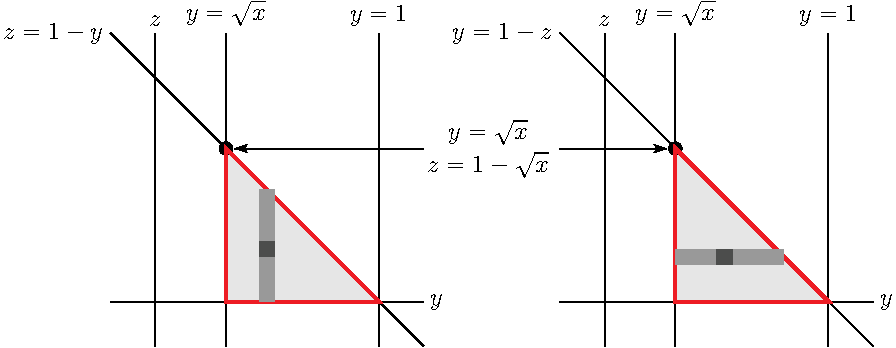
\includegraphics{OE08A_8x.pdf}
\end{center}
}
To reverse the order of the $y$-- and $z$--integrals we use 
horizontal strips as in the figure on the right above.
Looking at that figure, we see that, on $V_x$,
\begin{itemize}
\item
$z$ runs from $0$ to $1-\sqrt{x}$, and
\item
for each fixed $z$ in that range, $y$ runs from $\sqrt{x}$ to $1-z$.
\end{itemize}
So
\begin{align*}
I = \int_0^1\dee{x} \int_0^{1-\sqrt{x}}\dee{z} \int_{\sqrt{x}}^{1-z}\dee{y}
                \ f(x,y,z)
= \int_0^1 \int_0^{1-\sqrt{x}} \int_{\sqrt{x}}^{1-z}
                \ f(x,y,z)\  \dee{y}\,\dee{z}\,\dee{x}
\end{align*}

\bigskip
\emph{Outside integral is with respect to $y$}:\ \ \ 
Looking at the figures above we see that, for each $0\le x\le 1$,
$y$ runs from $\sqrt{x}$ to $1$ on $V_x$. As $x$ runs from $0$ to $1$ in $V$, 
we have that $\sqrt{x}$ also runs from $0$ to $1$ on $V$, so that
$y$ runs from $0$ to $1$ on $V$. Reviewing the definition of 
$V$, we see that, for each fixed $0\le y\le 1$, $(x,z)$ runs over
\begin{equation*}
V_y= \Set{(x,z)}{0\le x\le y^2,\ 0\le z\le 1-y}
\end{equation*} 
Here are two sketches of $V_y$.
\vadjust{
\begin{center}
     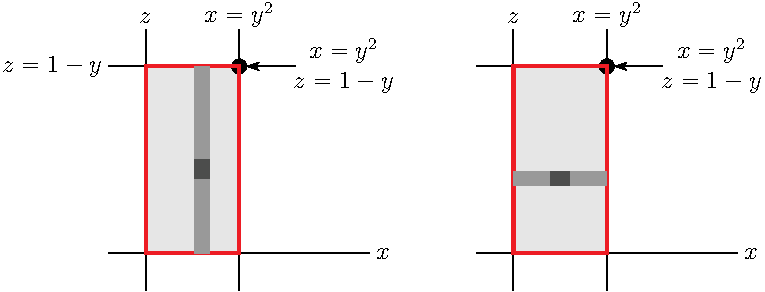
\includegraphics{OE08A_8y.pdf}
\end{center}
} 
Looking at the figure on the left (with the vertical strip), we see that, 
on $V_y$,
\begin{itemize}
\item 
$x$ runs from $0$ to $y^2$, and
\item 
for each fixed $x$ in that range,
$z$ runs from $0$ to $1-y$.
\end{itemize}
So
\begin{equation*}
I = \int_0^1 \dee{y} \int_0^{y^2}\dee{x} \int_0^{1-y}\dee{z}\ f(x,y,z)
  = \int_0^1  \int_0^{y^2}\int_0^{1-y}f(x,y,z)\ 
                   \dee{z}\,\dee{x}\, \dee{y}
\end{equation*}
Looking at the figure on the right above (with the horizontal strip), 
we see that, on $V_y$,
\begin{itemize}
\item 
$z$ runs from $0$ to $1-y$.
\item 
for each fixed $z$ in that range,
$x$ runs from $0$ to $y^2$.
\end{itemize}
So
\begin{equation*}
I = \int_0^1 \dee{y} \int_0^{1-y}\dee{z} \int_0^{y^2}\dee{x}\ f(x,y,z)
  = \int_0^1  \int_0^{1-y} \int_0^{y^2} f(x,y,z)\ 
                   \dee{x}\, \dee{z}\,\dee{y}
\end{equation*}
\bigskip


\emph{Outside integral is with respect to $z$}:\ \ \ 
Looking at the sketches of $V_x$ above we see that, for each $0\le x\le 1$,
$z$ runs from $0$ to $1-\sqrt{x}$ on $V_x$. As $x$ runs from $0$ to $1$ in
$V$, $1-\sqrt{x}$ also runs between $0$ to $1$ on $V$, so that $z$ 
runs from $0$ to $1$ on $V$.
Reviewing the definition of $V$, we see that,
for each fixed $0\le z\le 1$, $(x,y)$ runs over
\begin{equation*}
V_z= \Set{(x,y)}{0\le x\le y^2,\ \sqrt{x}\le y\le 1-z}
\end{equation*} 
Here are two sketches of $V_z$.
\vadjust{
\begin{center}
     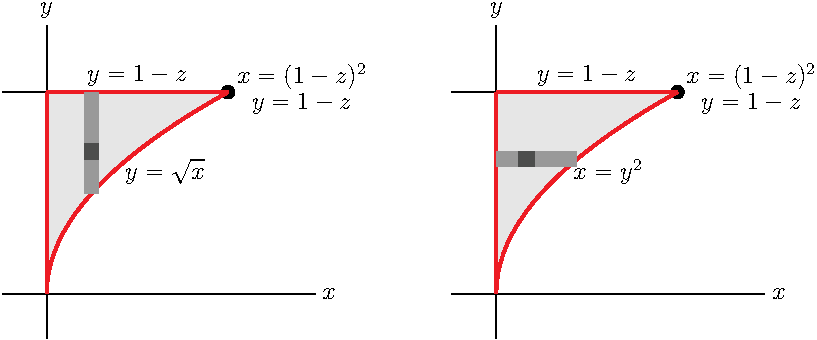
\includegraphics{OE08A_8z.pdf}
\end{center}
} 
Looking at the figure on the left (with the vertical strip), we see that, 
on $V_z$,
\begin{itemize}
\item 
$x$ runs from $0$ to $(1-z)^2$, and
\item 
for each fixed $x$ in that range,
$y$ runs from $\sqrt{x}$ to $1-z$.
\end{itemize}
So
\begin{equation*}
I = \int_0^1 \dee{z} \int_0^{(1-z)^2}\dee{x} \int_{\sqrt{x}}^{1-z}\dee{y}\ f(x,y,z)
  = \int_0^1  \int_0^{(1-z)^2} \int_{\sqrt{x}}^{1-z}f(x,y,z)\ 
                   \dee{y}\,\dee{x}\, \dee{z}
\end{equation*}
Looking at the figure on the right above (with the horizontal strip), 
we see that, on $V_z$,
\begin{itemize}
\item 
$y$ runs from $0$ to $1-z$.
\item 
for each fixed $y$ in that range,
$x$ runs from $0$ to $y^2$.
\end{itemize}
So
\begin{equation*}
I = \int_0^1 \dee{z} \int_0^{1-z}\dee{y} \int_0^{y^2}\dee{x}\ f(x,y,z)
  = \int_0^1  \int_0^{1-z} \int_0^{y^2} f(x,y,z)\ 
                   \dee{x}\, \dee{y}\,\dee{z}
\end{equation*}
\bigskip

\emph{Summary:}\ \ \ 
We have found that
\begin{alignat*}{3}
I&= \int_0^1 \int_{\sqrt{x}}^1 \int_0^{1-y} f(x,y,z)\,\dee{z}\,\dee{y}\,\dee{x}
&&=\int_0^1 \int_0^{1-\sqrt{x}} \int_{\sqrt{x}}^{1-z}
                \ f(x,y,z)\  \dee{y}\,\dee{z}\,\dee{x} \\
&=\int_0^1  \int_0^{y^2}\int_0^{1-y}f(x,y,z)\ 
                   \dee{z}\,\dee{x}\, \dee{y}
&&=\int_0^1  \int_0^{1-y} \int_0^{y^2} f(x,y,z)\ 
                   \dee{x}\, \dee{z}\,\dee{y} \\
&=\int_0^1  \int_0^{(1-z)^2} \int_{\sqrt{x}}^{1-z}f(x,y,z)\ 
                   \dee{y}\,\dee{x}\, \dee{z}
&&=\int_0^1  \int_0^{1-z} \int_0^{y^2} f(x,y,z)\ 
                   \dee{x}\, \dee{y}\,\dee{z}
\end{alignat*}

\end{solution}

%%%%%%%%%%%%%%%%%%%%%%%%%%%%%%%%
\begin{question}[M200 2009A] %8
Let $\displaystyle I = \tripInt_E f(x,y,z)\ \dee{V}$ 
where $E$ is the tetrahedron with vertices $(-1, 0, 0)$,
$(0, 0, 0)$, $(0, 0, 3)$ and $(0, -2, 0)$.


\begin{enumerate}[(a)]
\item
Rewrite the integral I in the form
\begin{equation*}
I = \int_{x=}^{x=}\int_{y=}^{y=}\int_{z=}^{z=} f(x,y,z)\ 
                                      \dee{z}\,\dee{y}\,\dee{x}
\end{equation*}

\item
Rewrite the integral I in the form
\begin{equation*}
I = \int_{z=}^{z=}\int_{x=}^{x=}\int_{y=}^{y=} f(x,y,z)\ 
                                      \dee{y}\,\dee{x}\,\dee{z}
\end{equation*}
\end{enumerate}
\end{question}

%\begin{hint}
%
%\end{hint}

\begin{answer}
(a) $I = \int_{x=-1}^{x=0}\int_{y=-2(1+x)}^{y=0}\int_{z=0}^{z=3(1+x+y/2)} 
            f(x,y,z)\ \dee{z}\,\dee{y}\,\dee{x}$

(b) $I = \int_{z=0}^{z=3}\int_{x=-(1-z/3)}^{x=0}\int_{y=-2(1+x-z/3)}^{y=0} 
             f(x,y,z)\ \dee{y}\,\dee{x}\,\dee{z}$
\end{answer}

\begin{solution}
First we have to get some idea as to what $E$ looks like.
Here is a sketch.
\begin{center}
     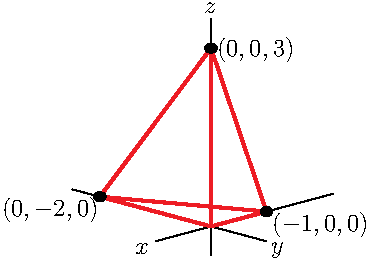
\includegraphics{OE09A_8.pdf}
\end{center}
We are going to need the equation of the plane that contains the
points $(-1,0,0)$, $(0,-2,0)$ and $(0,0,3)$. This plane does not contain
the origin and so has an equation of the form $ax+by+cz=1$. 
\begin{itemize}
\item
$(-1,0,0)$ lies on the plane $ax+by+cz=1$ if and only if
$a(-1)+b(0)+c(0)=1$. So $a=-1$.
\item
$(0,-2,0)$ lies on the plane $ax+by+cz=1$ if and only if
$a(0)+b(-2)+c(0)=1$. So $b=-\frac{1}{2}$.
\item
$(0,0,3)$ lies on the plane $ax+by+cz=1$ if and only if
$a(0)+b(0)+c(3)=1$. So $c=\frac{1}{3}$.
\end{itemize}
So the plane that contains the points $(-1,0,0)$, $(0,-2,0)$ and $(0,0,3)$
is $-x-\frac{y}{2}+\frac{z}{3}=1$.

We can now get a detailed mathematical description of $E$.
A point $(x,y,z)$ is in $E$ if and only if
\begin{itemize}
\item
$(x,y,z)$ lies above the $xy$--plane, i.e. $z\ge 0$, and
\item
$(x,y,z)$ lies to the left of the $xz$--plane, i.e. $y\le 0$, and
\item
$(x,y,z)$ lies behind the $yz$--plane, i.e. $x\le 0$, and
\item
$(x,y,z)$ lies on the same side of the plane 
$-x-\frac{y}{2}+\frac{z}{3}=1$ as the origin.
That is  $-x-\frac{y}{2}+\frac{z}{3}\le 1$. (Go ahead and check
that $(0,0,0)$ obeys this inequality.)

\end{itemize}
So
\begin{equation*}
E=\Set{(x,y,z)}{x\le 0,\ y\le 0,\ z\ge 0,\ -x-\tfrac{y}{2}+\tfrac{z}{3}\le 1}
\end{equation*}

(a) Note that we want the outside integral to be the $x$--integral.
On $E$
\begin{itemize}
\item 
$x$ runs from $-1$ to $0$ and
\item
for each fixed $x$ in that range $(y,z)$ runs over
\begin{align*}
E_x=\Set{(y,z)}{y\le 0,\ z\ge 0,\ -\tfrac{y}{2}+\tfrac{z}{3}\le 1+x}
\end{align*}
Here is a sketch of $E_x$.
\begin{center}
     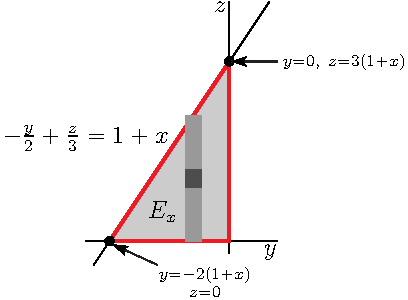
\includegraphics{OE09A_8a.pdf}
\end{center}

\item
On $E_x$, $y$ runs from $-2(1+x)$ to $0$ and
\item
for each fixed such $y$, $z$ runs from $0$ to $3(1+x+y/2)$
\end{itemize}
So
\begin{align*}
I = \int_{x=-1}^{x=0}\int_{y=-2(1+x)}^{y=0}\int_{z=0}^{z=3(1+x+y/2)} f(x,y,z)\ 
                                      \dee{z}\,\dee{y}\,\dee{x}
\end{align*}

(b) This time we want the outside integral to be the $z$--integral.
Looking back at the sketch of $E$, we see that, on $E$,
\begin{itemize}
\item 
$z$ runs from $0$ to $3$ and
\item
for each fixed $z$ in that range $(x,y)$ runs over
\begin{align*}
E_z=\Set{(x,y)}{x\le 0,\ y\le 0,\ -x-\tfrac{y}{2}\le 1-\tfrac{z}{3}}
\end{align*}
Here is a sketch of $E_z$.
\begin{center}
     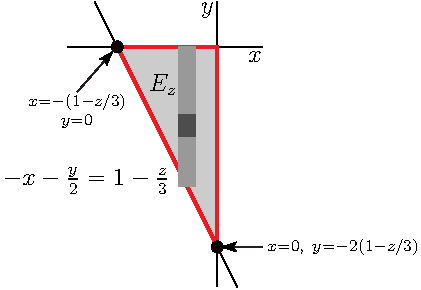
\includegraphics{OE09A_8b.pdf}
\end{center}

\item
On $E_z$, $x$ runs from $-(1-z/3)$ to $0$ and
\item
for each fixed such $x$, $y$ runs from $-2(1+x-z/3)$ to $0$
\end{itemize}
So
\begin{align*}
I = \int_{z=0}^{z=3}\int_{x=-(1-z/3)}^{x=0}\int_{y=-2(1+x-z/3)}^{y=0} f(x,y,z)\ 
                                      \dee{y}\,\dee{x}\,\dee{z}
\end{align*}
\end{solution}

%%%%%%%%%%%%%%%%%%%%%%%%%%%%%%%%
\begin{question}[M200 2010D] %7
Let $T$ denote the tetrahedron bounded by the coordinate planes $x = 0$, $y = 0$, $z = 0$ and
the plane $x + y + z = 1$. Compute
\begin{equation*}
K = \tripInt_T \frac{1}{ (1 + x + y + z)^4}\ \dee{V}
\end{equation*}
\end{question}

%\begin{hint}
%
%\end{hint}

\begin{answer}
$\frac{1}{48}$
\end{answer}

\begin{solution}
The plane $x+y+z=1$ intersects the coordinate plane $z=0$
along the line $x+y=1$, $z=0$. So
\begin{align*}
T&=\Set{(x,y,z)}{x\ge 0,\  y\ge0,\ x+y\le 1,\ 0\le z\le 1-x-y} \\
 &=\Set{(x,y,z)}{0\le x\le 1,\  0\le y\le 1-x,\ 0\le z\le 1-x-y}
\end{align*}
\begin{center}
     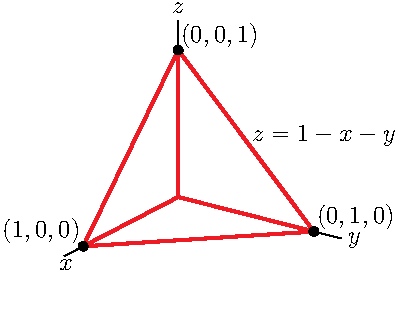
\includegraphics{OE10D_7.pdf}
\end{center}
and
\begin{align*}
K&=\int_0^1\dee{x}\int_0^{1-x}\dee{y}\int_0^{1-x-y}\dee{z}\ 
           \frac{1}{ (1 + x + y + z)^4} \\[0.1in]
&=\int_0^1\dee{x}\int_0^{1-x}\dee{y}\ 
           \left[-\frac{1}{ 3(1 + x + y + z)^3}\right]_{z=0}^{z=1-x-y} \\[0.1in]
&=\frac{1}{3}\int_0^1\dee{x}\int_0^{1-x}\dee{y}\ 
           \left[\frac{1}{(1 + x + y)^3} - \frac{1}{2^3}\right] \\[0.1in]
&=\frac{1}{3}\int_0^1\dee{x}\ 
    \left[-\frac{1}{2(1 + x + y)^2} - \frac{y}{2(4)}\right]_{y=0}^{y=1-x} \\[0.1in]
&=\frac{1}{6}\int_0^1\dee{x}\ 
    \left[\frac{1}{(1 + x)^2}-\frac{1}{2^2}- \frac{1-x}{4}\right]
=\frac{1}{6}\int_0^1\dee{x}\ 
    \left[\frac{1}{(1 + x)^2} -\frac{1}{2} + \frac{x}{4}\right] \\[0.1in]
&=\frac{1}{6} 
    \left[-\frac{1}{1 + x} -\frac{x}{2} + \frac{x^2}{8}\right]_{x=0}^{x=1}
=\frac{1}{6} 
    \left[1-\frac{1}{2} -\frac{1}{2} + \frac{1}{8}\right] \\[0.1in]
&=\frac{1}{48}
\end{align*}
\end{solution}

%%%%%%%%%%%%%%%%%%%%%%%%%%%%%%%%
\begin{question}[M200 2011A] %7
Let $E$ be the portion of the first octant which is above the plane $z = x + y$ 
and below the plane $z = 2$. The density in $E$ is $\rho(x, y, z) = z$. Find the mass of $E$.
\end{question}

%\begin{hint}
%
%\end{hint}

\begin{answer}
$2$
\end{answer}

\begin{solution}
Note that the planes $z = x + y$ and $z = 2$ intersect along the line
$x+y=2$, $z=2$. 

\begin{center}
     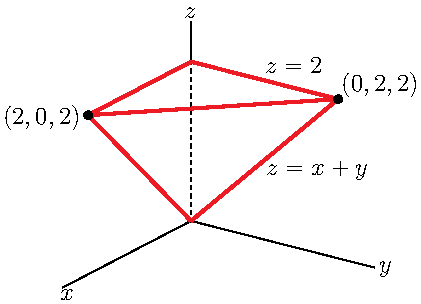
\includegraphics[scale=1.0]{OE11A_7.pdf}
\end{center}

So
\begin{align*}
E &=\Set{(x,y,z)}{x\ge 0,\ y\ge 0,\ x+y\le 2,\ x+y\le z\le 2} \\
  &= \Set{(x,y,z)}{0\le x\le 2,\ 0\le y\le 2-x,\ x+y\le z\le 2} 
\end{align*}
and the mass of $E$ is
\begin{align*}
\tripInt_E \rho(x,y,z)\,\dee{V}
&=\int_0^2\dee{x} \int_0^{2-x}\dee{y} \int_{x+y}^2\dee{z}\ z \\
&=\frac{1}{2}\int_0^2\dee{x} \int_0^{2-x}\dee{y} \ \big[4-(x+y)^2\big] \\
&=\frac{1}{2}\int_0^2\dee{x}\ 
              \left[4(2-x)-\frac{\big(x+(2-x)\big)^3-x^3}{3}\right] \\
&=\frac{1}{2}  \left[4(2)(2)-2(2)^2 -\frac{8}{3}(2)+\frac{2^4}{12}
              \right]
=\frac{1}{2}  \left[8 -\frac{16}{3}+\frac{4}{3}
              \right] \\
&=2
\end{align*}
\end{solution}

%%%%%%%%%%%%%%%%%%%%%%%%%%%%%%%%
\begin{question}[M200 2011D] %7
Evaluate the triple integral $\tripInt_E x\ \dee{V}$, where $E$ is 
the region in the first octant bounded by the parabolic cylinder $y = x^2$ 
and the planes $y + z = 1$, $x = 0$, and $z = 0$.
\end{question}

%\begin{hint}
%
%\end{hint}

\begin{answer}
$\frac{1}{12}$
\end{answer}

\begin{solution}
First, we need to develop an understanding of what $E$ looks like.
Here are sketches of the parabolic cylinder $y=x^2$, on the left,
and the plane $y+z=1$, on the right.
\begin{center}
     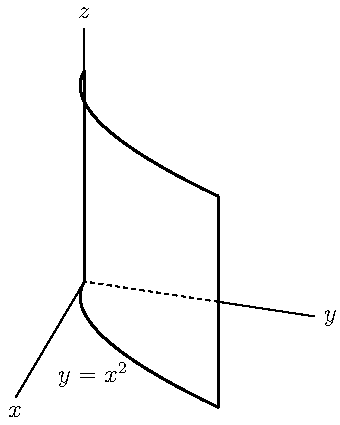
\includegraphics[scale=0.9]{OE11D_7b.pdf}\qquad
     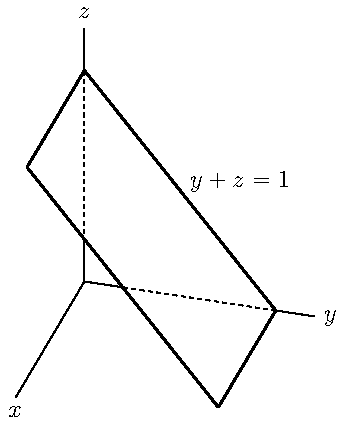
\includegraphics[scale=0.9]{OE11D_7a.pdf}
\end{center}
$E$ is constructed by using the plane $y+z=1$ to chop the top
off of the parabolic cylinder $y=x^2$. Here is a sketch.
\begin{center}
     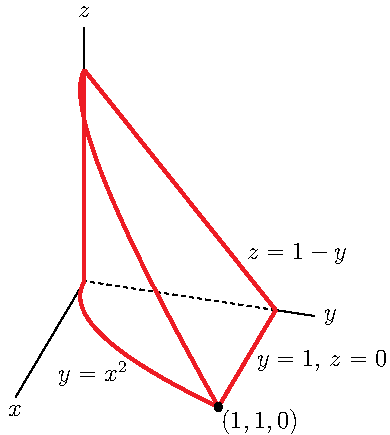
\includegraphics{OE11D_7c.pdf}
\end{center}
So
\begin{equation*}
E=\Set{(x,y,z)}{0\le x\le 1,\ x^2\le y\le 1,\ 0\le z\le 1-y}
\end{equation*}
and the integral
\begin{align*}
\tripInt_E x\ \dee{V}
&=\int_0^1\dee{x}\int_{x^2}^1\dee{y}\int_0^{1-y}\dee{z}\ x \\
&=\int_0^1\dee{x}\int_{x^2}^1\dee{y}\ x(1-y) \\
&=\int_0^1\dee{x}\ x\left[y-\frac{y^2}{2}\right]_{x^2}^1 \\
&=\int_0^1\dee{x}\ \left[\frac{x}{2} -x^3+\frac{x^5}{2}\right] \\
&=\frac{1}{4}-\frac{1}{4}+\frac{1}{12} \\
&=\frac{1}{12}
\end{align*} 
\end{solution}

%%%%%%%%%%%%%%%%%%%%%%%%%%%%%%%%
\begin{question}[M200 2012A] %8
Let $E$ be the region in the first octant bounded by the coordinate planes, 
the plane $x + y = 1$ and the surface $z = y^2$ .  Evaluate
$\tripInt_E z\ \dee{V}$ .
\end{question}

%\begin{hint}
%
%\end{hint}

\begin{answer}
$\frac{1}{60}$
\end{answer}

\begin{solution}
First, we need to develop an understanding of what $E$ looks like.
Here are sketches of the plane $x+y=1$, on the left, and of the ``tower''
bounded by the coordinate planes $x=0$, $y=0$, $z=0$ and the
plane $x+y=1$, on the right.
\begin{center}
     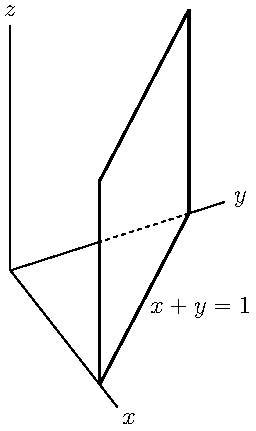
\includegraphics{OE12A_8a.pdf}\qquad
     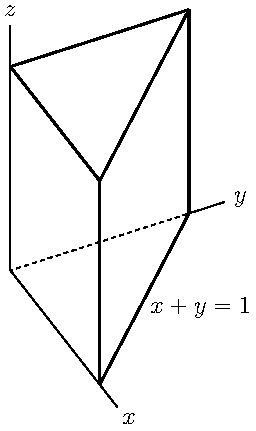
\includegraphics{OE12A_8aa.pdf}
\end{center}
Now here is the parabolic cylinder $z=y^2$ on the left.
$E$ is constructed by using the parabolic cylinder $z=y^2$ to chop the top
off of the tower $x\ge 0$, $y\ge 0$, $z\ge 0$,  $x+y\le 1$. The figure 
on the right is a sketch.
\begin{center}
     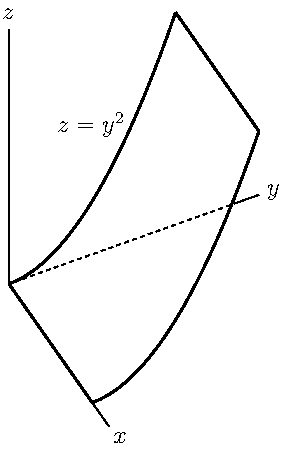
\includegraphics{OE12A_8b.pdf}\qquad
     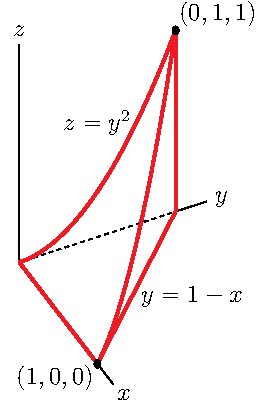
\includegraphics{OE12A_8c.pdf}
\end{center}
So
\begin{equation*}
E=\Set{(x,y,z)}{0\le x\le 1,\ 0\le y\le 1-x,\ 0\le z\le y^2}
\end{equation*}
and the integral
\begin{align*}
\tripInt_E z\ \dee{V}
&=\int_0^1\dee{x}\int_0^{1-x}\dee{y}\int_0^{y^2}\dee{z}\ z \\
&=\int_0^1\dee{x}\int_0^{1-x}\dee{y}\ \frac{y^4}{2} \\
&=\int_0^1\dee{x}\ \frac{(1-x)^5}{10} \\
&=\left[-\frac{(1-x)^6}{60}\right]_0^1 \\
&=\frac{1}{60}
\end{align*} 
\end{solution}

%%%%%%%%%%%%%%%%%%%%%%%%%%%%%%%%
\begin{question}[M200 2012D] %9
Evaluate  $\tripInt_R yz^2 e^{-xyz}\ \dee{V}$ over the rectangular
box
\begin{equation*}
R=\Set{(x,y,z)}{0\le x\le 1,\ 0\le y\le 2,\  0\le z\le 3}
\end{equation*} 
\end{question}

%\begin{hint}
%
%\end{hint}

\begin{answer}
$\frac{13}{2}-\frac{e^{-6}}{2}$
\end{answer}

\begin{solution}
The integral
\begin{align*}
\tripInt_R yz^2 e^{-xyz}\ \dee{V}
&=\int_0^3\dee{z}\int_0^2\dee{y}\int_0^1\dee{x}\ yz^2 e^{-xyz} \\
&=\int_0^3\dee{z}\int_0^2\dee{y}\ \Big[-z e^{-xyz}\Big]_{x=0}^{x=1} 
  =\int_0^3\dee{z}\int_0^2\dee{y}\ \Big[z-z e^{-yz}\Big] \\
&=\int_0^3\dee{z}\ \Big[zy+ e^{-yz}\Big]_{y=0}^{y=2}
=\int_0^3\dee{z}\ \Big[2z+ e^{-2z}-1\Big] \\
&=\left[z^2-\frac{1}{2} e^{-2z}-z\right]_0^3 
=\frac{13}{2}-\frac{e^{-6}}{2}
\end{align*}
\end{solution}

\begin{question}[M200 2013D] %8
\begin{enumerate}[(a)]
\item
Sketch the surface given by the equation $z = 1 - x^2$.
\item
Let $E$ be the solid bounded by the plane $y = 0$, the cylinder 
$z = 1 - x^2$, and the plane $y = z$. Set up the integral
\begin{equation*}
\tripInt_E f(x,y,z)\,\dee{V}
\end{equation*}
as an iterated integral.
\end{enumerate}
\end{question}

%\begin{hint}
%
%\end{hint}

\begin{answer}
(a)
\begin{center}
     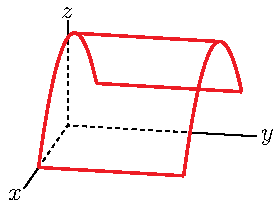
\includegraphics{OE13D_8.pdf}
\end{center}

(b) $\int_{-1}^1\dee{x}\int_0^{1-x^2}\dee{y}\int_y^{1-x^2}\dee{z}\ f(x,y,z)$
\end{answer}

\begin{solution}
(a)
Each constant $y$ cross section of $z=1-x^2$ is an upside
down parabola. So the surface is a bunch of upside down parabolas
stacked side by side. The figure on the left below is a sketch of 
the part of the surface with $y\ge 0$
and $z\ge 0$ (both of which conditions will be required in part (b)).

\begin{center}
     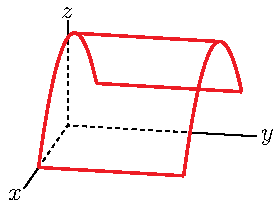
\includegraphics{OE13D_8.pdf}\qquad
     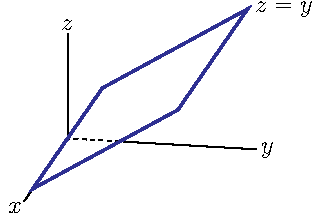
\includegraphics{OE13D_8b1.pdf}
\end{center}

(b)
The figure on the right above is a sketch of the plane $y=z$.
It intersects the surface $z=1-x^2$ in the solid blue sloped parabolic
curve in the figure below.

\begin{center}
     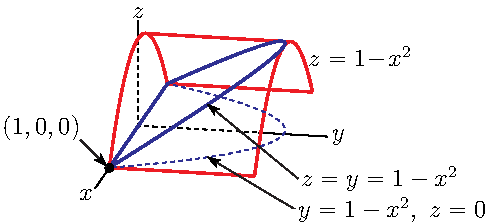
\includegraphics{OE13D_8b3.pdf}
\end{center}

Observe that, on the curve $z=1-x^2$, $z=y$, we have
$y=1-x^2$. So that when one looks at the solid $E$ from high on the $z$--axis,
one sees
\begin{equation*}
\Set{(x,y)}{0\le y\le 1-x^2}
\end{equation*} 
The $y=1-x^2$ boundary of that region is the dashed blue line in the 
$xy$--plane in the figure above. So 
\begin{equation*}
E = \Set{(x,y,z)}{-1\le x\le 1,\ 0\le y\le 1-x^2,\ y\le z\le 1-x^2}
\end{equation*}
and the integral
\begin{equation*}
\tripInt_E f(x,y,z)\,\dee{V}
=\int_{-1}^1\dee{x}\int_0^{1-x^2}\dee{y}\int_y^{1-x^2}\dee{z}\ f(x,y,z)
\end{equation*}
\end{solution}

\begin{question}[M200 2014A] %6b
Let
\begin{equation*}
J=\int_0^1 \int_0^x\int_0^y f(x,y,z)\ \dee{z}\,\dee{y}\,\dee{x}
\end{equation*}
Express $J$ as an integral where the integrations are to be performed 
in the order $x$ first, then $y$, then $z$.
\end{question}

%\begin{hint}
%
%\end{hint}

\begin{answer}
$J = \int_0^1 \int_z^1\int_y^1 f(x,y,z)\ \dee{x}\,\dee{y}\,\dee{z}$
\end{answer}

\begin{solution}
In the integral $J$,
\begin{itemize}
\item
$x$ runs from $0$ to $1$. 
In inequalities, $0\le x\le 1$.
\item
Then, for each fixed $x$ in that range, $y$ runs from $0$ to $x$.
In inequalities, $0\le y\le x$.
\item
Then, for each fixed $x$ and $y$ in those ranges, $z$ runs from $0$ to $y$.
In inequalities, $0\le z\le y$.

\end{itemize}
These inequalties can be combined into 
\begin{equation*}
0\le z\le y\le x\le 1 \tag{$*$}
\end{equation*}
We wish to reverse the order of integration so that the $z$--integral
is on the outside, the $y$--integral is in the middle and the $x$--integral
is on the inside.
\begin{itemize}
\item
The smallest $z$ compatible with $(*)$ is $z=0$
and the largest $z$ compatible with $(*)$ is $z=1$ (when $x=y=z=1$).
So $0\le z\le 1$.
\item
Then, for each fixed $z$ in that range, $(x,y)$ run over 
$z\le y\le x\le 1$. In particular, the smallest allowed $y$ is $y=z$
and the largest allowed $y$ is $y=1$ (when $x=y=1$).
So $z\le y\le 1$.
\item
Then, for each fixed $y$ and $z$ in those ranges, $x$ runs over 
$y\le x\le 1$.
\end{itemize}
So 
\begin{equation*}
J = \int_0^1 \int_z^1\int_y^1 f(x,y,z)\ \dee{x}\,\dee{y}\,\dee{z}
\end{equation*}
\end{solution}


\begin{question}[M200 2014D] %9
Let $E$ be the region bounded by $z = 2x$, $z = y^2$, and $x = 3$. 
The triple integral $\tripInt f(x,y,z)\,\dee{V}$ can be expressed 
as an iterated integral in the following three orders
of integration. Fill in the limits of integration in each case. 
No explanation required.
\begin{align*}
&\int_{y=}^{y=}\qquad\int_{x=}^{x=}\qquad\int_{z=}^{z=}\qquad
                f(x,y,z)\ \dee{z}\,\dee{x}\,\dee{y} \\[0.1in]
&\int_{y=}^{y=}\qquad\int_{z=}^{z=}\qquad\int_{x=}^{x=}\qquad
                f(x,y,z)\ \dee{x}\,\dee{z}\,\dee{y} \\[0.1in]
&\int_{z=}^{z=}\qquad\int_{x=}^{x=}\qquad\int_{y=}^{y=}\qquad
                f(x,y,z)\ \dee{y}\,\dee{x}\,\dee{z} 
\end{align*}
\end{question}

%\begin{hint}
%
%\end{hint}

\begin{answer}
$\int_{y=-\sqrt{6}}^{y=\sqrt{6}}\int_{x=y^2/2}^{x=3}\int_{z=y^2}^{z=2x}
                f(x,y,z)\ \dee{z}\,\dee{x}\,\dee{y}$

$\int_{y=-\sqrt{6}}^{y=\sqrt{6}}\int_{z=y^2}^{z=6}\int_{x=z/2}^{x=3}
                f(x,y,z)\ \dee{x}\,\dee{z}\,\dee{y}$

$\int_{z=0}^{z=6}\int_{x=z/2}^{x=3}\int_{y=-\sqrt{z}}^{y=\sqrt{z}}
                f(x,y,z)\ \dee{y}\,\dee{x}\,\dee{z}$
\end{answer}

\begin{solution}
The hard part of this problem is figuring out what $E$ looks like.
First here are separate sketches of the plane $x=3$ and the plane
$z=2x$ followed by a sketch of the two planes together.

\begin{center}
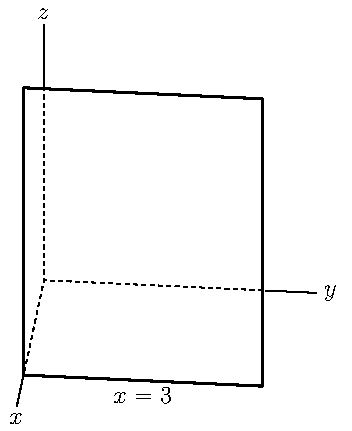
\includegraphics[scale=0.7]{OE14D_9a.pdf}\qquad
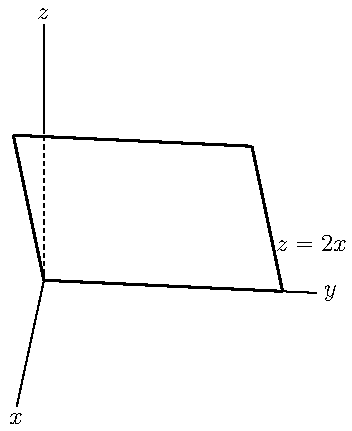
\includegraphics[scale=0.7]{OE14D_9b.pdf}\qquad
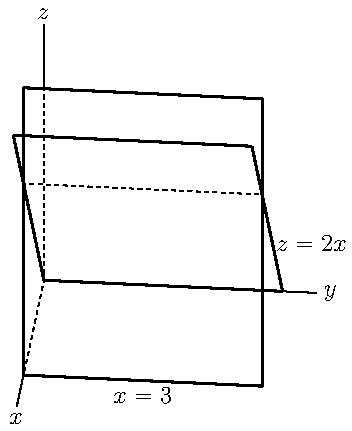
\includegraphics[scale=0.7]{OE14D_9c.pdf}
\end{center} 

Next for the parabolic cylinder $z=y^2$. 
It is a bunch of parabolas $z=y^2$ stacked side by side along the $x$--axis. Here is a sketch of the part of  $z=y^2$ in the first octant.

\begin{center}
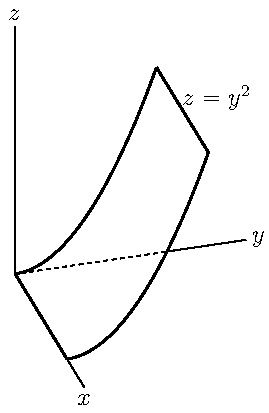
\includegraphics[scale=0.7]{OE14D_9d.pdf}
\end{center} 

Finally, here is a sketch of the part of $E$ in the first octant.
$E$ does have a second half gotten from the sketch by reflecting it
in the $xz$--plane, i.e. by replacing $y\rightarrow-y$.

\begin{center}
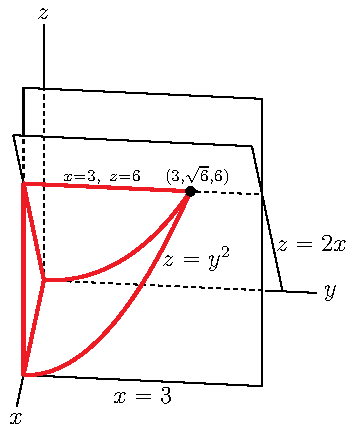
\includegraphics{OE14D_9.pdf}
\end{center} 

So\footnote{The question doesn't specify on which side of the three surfaces
$E$ lies. When in doubt take the finite region bounded by the given surfaces.
That's what we have done.}
\begin{equation*}
E = \Set{(x,y,z)}{x\le 3,\ -\sqrt{6}\le y\le \sqrt{6},\ y^2\le z\le 2x}
\end{equation*}

\emph{Order $\dee{z}\,\dee{x}\,\dee{y}$:\ \ \ }
On $E$, $y$ runs from $-\sqrt{6}$ to $\sqrt{6}$. For each fixed $y$
in this range $(x,z)$ runs over $E_y=\Set{(x,z)}{x\le 3,\ y^2\le z\le 2x}$.
Here is a sketch of $E_y$.

\begin{center}
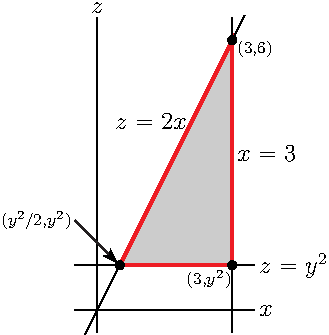
\includegraphics{OE14D_9e.pdf}
\end{center} 

From the sketch
\begin{equation*}
E_y = \Set{(x,z)}{y^2/2\le x\le 3,\ y^2\le z\le 2x}
\end{equation*}
and the integral is
\begin{equation*}
\int_{y=-\sqrt{6}}^{y=\sqrt{6}}\int_{x=y^2/2}^{x=3}\int_{z=y^2}^{z=2x}
                f(x,y,z)\ \dee{z}\,\dee{x}\,\dee{y} 
\end{equation*} 


\emph{Order $\dee{x}\,\dee{z}\,\dee{y}$:\ \ \ }
Also from the sketch of $E_y$ above
\begin{equation*}
E_y = \Set{(x,z)}{y^2\le z\le 6,\ z/2\le x\le 3}
\end{equation*}
and the integral is
\begin{equation*}
\int_{y=-\sqrt{6}}^{y=\sqrt{6}}\int_{z=y^2}^{z=6}\int_{x=z/2}^{x=3}
                f(x,y,z)\ \dee{x}\,\dee{z}\,\dee{y} 
\end{equation*} 


\emph{Order $\dee{y}\,\dee{x}\,\dee{z}$:\ \ \ }
From the sketch of the part of $E$ in the first octant, we see that,
on $E$, $z$ runs from $0$ to $6$. For each fixed $z$
in this range $(x,y)$ runs over 
\begin{align*}
E_z&=\Set{(x,y)}{x\le 3,\ -\sqrt{6}\le y\le \sqrt{6},\ y^2\le z\le 2x} \\
&=\Set{(x,y)}{z/2\le x\le 3,\ y^2\le z} \\
&=\Set{(x,y)}{z/2\le x\le 3,\ -\sqrt{z}\le y\le \sqrt{z} } 
\end{align*}
So the integral is
\begin{equation*}
\int_{z=0}^{z=6}\int_{x=z/2}^{x=3}\int_{y=-\sqrt{z}}^{y=\sqrt{z}}
                f(x,y,z)\ \dee{y}\,\dee{x}\,\dee{z} 
\end{equation*}
\end{solution}

%%%%%%%%%%%%%%%%%%%%%%%%%%%%%%%%
\begin{question}[M200 2015D] %7
Let E be the region inside the cylinder $x^2 + y^2 = 1$, 
below the plane $z = y$ and above the plane $z = -1$. Express 
the integral
\begin{equation*}
\tripInt_E f(x,y,z)\ \dee{V}
\end{equation*}
as three different iterated integrals corresponding to the orders 
of integration: (a) $\dee{z}\, \dee{x}\, \dee{y}$,
(b) $\dee{x}\, \dee{y}\, \dee{z}$, and (c) $\dee{y}\, \dee{z}\, \dee{x}$.
\end{question}

%\begin{hint}
%
%\end{hint}

\begin{answer}
(a) $\int_{-1}^1\int_{-\sqrt{1-y^2}}^{\sqrt{1-y^2}}
        \int_{-1}^y f(x,y,z)\ \dee{z}\,\dee{x}\,\dee{y} $\qquad
(b) $\int_{-1}^1\int_z^1 \int_{-\sqrt{1-y^2}}^{\sqrt{1-y^2}}
              f(x,y,z)\ \dee{x}\,\dee{y}\,\dee{z}$

(c) $\int_{-1}^1 \int_{-1}^{-\sqrt{1-x^2}} \int_{-\sqrt{1-x^2}}^{\sqrt{1-x^2}}
              f(x,y,z)\ \dee{y}\,\dee{z}\,\dee{x}
       +\int_{-1}^1 \int_{-\sqrt{1-x^2}}^{\sqrt{1-x^2}}
                    \int_z^{\sqrt{1-x^2}}  f(x,y,z)\ \dee{y}\,\dee{z}\,\dee{x}$
\end{answer}

\begin{solution}
(a)
The region $E$ is
\begin{align*}
E &= \Set{(x,y,z)}{x^2+y^2\le 1,\ -1\le z\le y} 
\end{align*}
Here is are sketches, one without axes and one with axes, 
of the front half of $E$, outlined in red.

\begin{center}
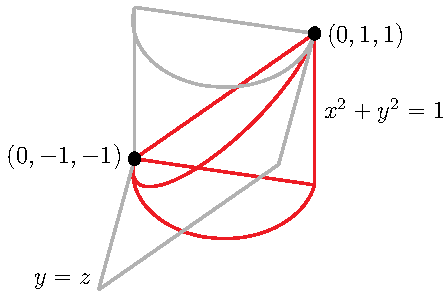
\includegraphics{OE15D_7A.pdf}\quad
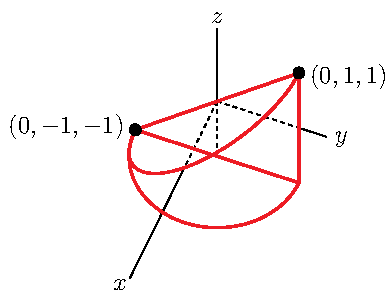
\includegraphics{OE15D_7AA.pdf}
\end{center}

The integral
\begin{align*}
\tripInt_E f(x,y,z)\ \dee{V}
&=\int_{x^2+y^2\le 1}\dee{x}\,\dee{y}\int_{-1}^y\dee{z}\ f(x,y,z) \\
&=\int_{-1}^1\dee{y}\int_{-\sqrt{1-y^2}}^{\sqrt{1-y^2}}\dee{x}
        \int_{-1}^y\dee{z}\ f(x,y,z) \\
&=\int_{-1}^1\int_{-\sqrt{1-y^2}}^{\sqrt{1-y^2}}
        \int_{-1}^y f(x,y,z)\ \dee{z}\,\dee{x}\,\dee{y} 
\end{align*}



(b)
Here is a sketch of (the front half of) a constant $z$  slice of $E$.

\begin{center}
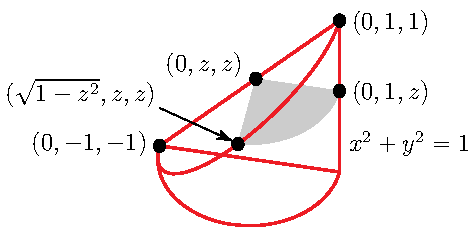
\includegraphics{OE15D_7B.pdf}
\end{center}

Note that
\begin{itemize}
\item
  in $E$, $z$ runs from $-1$ to $1$.
\item 
  Once $z$ has been fixed, $x$ and $y$ must obey $x^2+y^2\le 1$,
     $z\le y\le 1$
\end{itemize}
So 
\begin{align*}
E &= \Set{(x,y,z)}{-1\le z\le 1,\ z\le y\le 1,\ 
            -\sqrt{1-y^2}\le x\le\sqrt{1-y^2}} 
\end{align*}
and 
\begin{align*}
\tripInt_E f(x,y,z)\ \dee{V}
&=\int_{-1}^1\dee{z}\int_z^1\dee{y}
         \int_{-\sqrt{1-y^2}}^{\sqrt{1-y^2}}\dee{x}\ f(x,y,z) \\
&=\int_{-1}^1\int_z^1 \int_{-\sqrt{1-y^2}}^{\sqrt{1-y^2}}
              f(x,y,z)\ \dee{x}\,\dee{y}\,\dee{z} 
\end{align*}


(c)
Here is a sketch of a constant $x$  slice of $E$.

\begin{center}
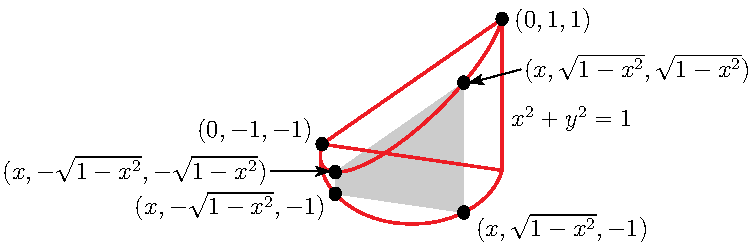
\includegraphics{OE15D_7C.pdf}
\end{center}

Note that
\begin{itemize}
\item
  in $E$, $x$ runs from $-1$ to $1$.
\item 
  Once $x$ has been fixed, $y$ and $z$ must obey
   \begin{equation*}
       -\sqrt{1-x^2}\le y\le\sqrt{1-x^2}\qquad -1\le z\le y 
   \end{equation*}
\end{itemize}
Here is a sketch.
\begin{center}
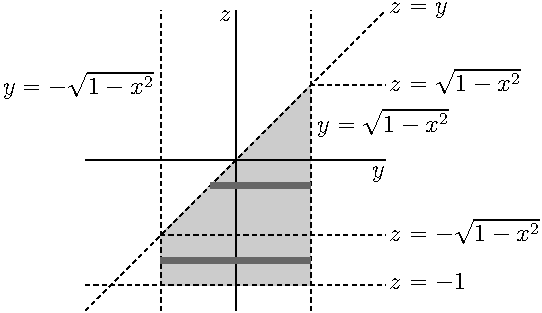
\includegraphics{OE15D_7CC.pdf}
\end{center}
Note that
\begin{itemize}
\item
    $z$ runs from $-1$ to  $\sqrt{1-x^2}$.
\item
    For each $z$ between $-1$ and $-\sqrt{1-x^2}$, $y$ runs from 
    $-\sqrt{1-x^2}$ to $\sqrt{1-x^2}$, while
\item
    for each $z$ between $-\sqrt{1-x^2}$ and $\sqrt{1-x^2}$, $y$ runs from 
    $z$ to $\sqrt{1-x^2}$.
\end{itemize}
So 
\begin{align*}
\tripInt_E f(x,y,z)\ \dee{V}
&=\int_{-1}^1\dee{x} \int_{-1}^{-\sqrt{1-x^2}}\dee{z}  
                     \int_{-\sqrt{1-x^2}}^{\sqrt{1-x^2}}\dee{y}  \ f(x,y,z) \\
&\hskip1in  +\int_{-1}^1\dee{x} \int_{-\sqrt{1-x^2}}^{\sqrt{1-x^2}}\dee{z}  
                    \int_z^{\sqrt{1-x^2}}\dee{y}  \ f(x,y,z) 
\end{align*}
or
\begin{align*}
\tripInt_E f(x,y,z)\ \dee{V}
&=\int_{-1}^1 \int_{-1}^{-\sqrt{1-x^2}} \int_{-\sqrt{1-x^2}}^{\sqrt{1-x^2}}
              f(x,y,z)\ \dee{y}\,\dee{z}\,\dee{x} \\
&\hskip1in  +\int_{-1}^1 \int_{-\sqrt{1-x^2}}^{\sqrt{1-x^2}}
                    \int_z^{\sqrt{1-x^2}}  f(x,y,z)\ \dee{y}\,\dee{z}\,\dee{x} 
\end{align*}
\end{solution}


%%%%%%%%%%%%%%%%%%%%%%%%%%%%%%%%
\begin{question}[M200 2016D] %8
Let $E$ be the region bounded by the planes $y=0$, $y=2$,
$y+z=3$ and the surface $z=x^2$. Consider the intergal
\begin{align*}
I=\tripInt_E f(x,y,z)\ \dee{V}
\end{align*}
Fill in the blanks below. In each part below,
you may need only one integral to express your answer. In that
case, leave the other blank.

\begin{enumerate}[(a)]
\item
$\displaystyle I=\int_{\underline{\ \ \ \ }}^{\underline{\ \ \ \ }}
                 \int_{\underline{\ \ \ \ }}^{\underline{\ \ \ \ }}
                 \int_{\underline{\ \ \ \ }}^{\underline{\ \ \ \ }}
                        f(x,y,z)\ \dee{z}\,\dee{x}\,\dee{y} +
                 \int_{\underline{\ \ \ \ }}^{\underline{\ \ \ \ }}
                 \int_{\underline{\ \ \ \ }}^{\underline{\ \ \ \ }}
                 \int_{\underline{\ \ \ \ }}^{\underline{\ \ \ \ }}
                        f(x,y,z)\ \dee{z}\,\dee{x}\,\dee{y} $
\medskip
\item
$\displaystyle I=\int_{\underline{\ \ \ \ }}^{\underline{\ \ \ \ }}
                 \int_{\underline{\ \ \ \ }}^{\underline{\ \ \ \ }}
                 \int_{\underline{\ \ \ \ }}^{\underline{\ \ \ \ }}
                        f(x,y,z)\ \dee{x}\,\dee{y}\,\dee{z} +
                 \int_{\underline{\ \ \ \ }}^{\underline{\ \ \ \ }}
                 \int_{\underline{\ \ \ \ }}^{\underline{\ \ \ \ }}
                 \int_{\underline{\ \ \ \ }}^{\underline{\ \ \ \ }}
                        f(x,y,z)\ \dee{x}\,\dee{y}\,\dee{z} $
\medskip
\item
$\displaystyle I=\int_{\underline{\ \ \ \ }}^{\underline{\ \ \ \ }}
                 \int_{\underline{\ \ \ \ }}^{\underline{\ \ \ \ }}
                 \int_{\underline{\ \ \ \ }}^{\underline{\ \ \ \ }}
                        f(x,y,z)\ \dee{y}\,\dee{x}\,\dee{z} +
                 \int_{\underline{\ \ \ \ }}^{\underline{\ \ \ \ }}
                 \int_{\underline{\ \ \ \ }}^{\underline{\ \ \ \ }}
                 \int_{\underline{\ \ \ \ }}^{\underline{\ \ \ \ }}
                        f(x,y,z)\ \dee{y}\,\dee{x}\,\dee{z} $

\end{enumerate}
\end{question}

%\begin{hint}
%
%\end{hint}

\begin{answer}
(a) $\int_0^2 \int_{-\sqrt{3-y}}^{\sqrt{3-y}} \int_{x^2}^{3-y} 
                 f(x,y,z)\ \dee{z}\,\dee{x}\,\dee{y}$

(b) $\int_0^1 \int_0^2 \int_{-\sqrt{z}}^{\sqrt{z}} f(x,y,z)\    
                 \dee{x}\,\dee{y}\,\dee{z}
     +\int_1^3 \int_0^{3-z} \int_{-\sqrt{z}}^{\sqrt{z}} f(x,y,z)\    
                 \dee{x}\,\dee{y}\,\dee{z}$

(c) $\int_0^1  \int_{-\sqrt{z}}^{\sqrt{z}}\int_0^2 f(x,y,z)\    
                 \dee{y}\,\dee{x}\,\dee{z}
    +\int_1^3 \int_{-\sqrt{z}}^{\sqrt{z}}  \int_0^{3-z} f(x,y,z)\    
                 \dee{y}\,\dee{x}\,\dee{z}$
\end{answer}

\begin{solution}
First, we need to develop an understanding of what $E$ looks like.
Note that all of the equations $y=0$, $y=2$, $y+z=3$ and $z=x^2$
are invariant under $x\rightarrow -x$. So $E$ is invariant under 
$x\rightarrow -x$, i.e. is symmetric about the $yz$--plane. We'll sketch
the first octant (i.e. $x,y,z\ge 0$) part of $E$. There is also a
$x\le 0$, $y\ge 0$, $z\ge 0$ part.

Here are sketches of the plane $y=2$, on the left, 
the plane $y+z=3$ in the centre and of the ``tunnel''
bounded by the coordinate planes $x=0$, $y=0$, $z=0$ and the
planes $y=2$, $y+z=3$, on the right.
\begin{center}
     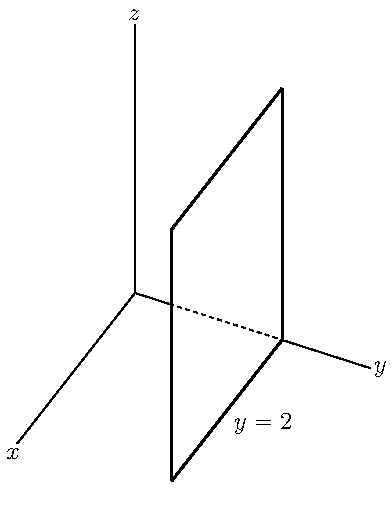
\includegraphics[scale=0.7]{OE16D_8a.pdf}\quad 
     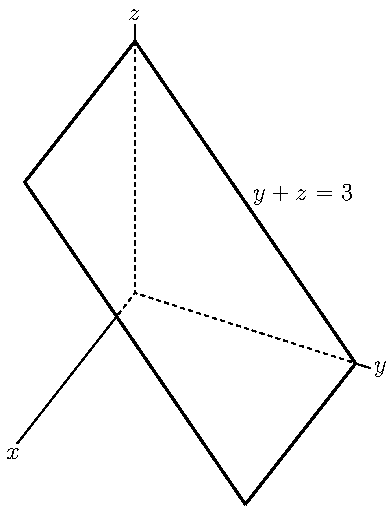
\includegraphics[scale=0.7]{OE16D_8b.pdf}\quad 
     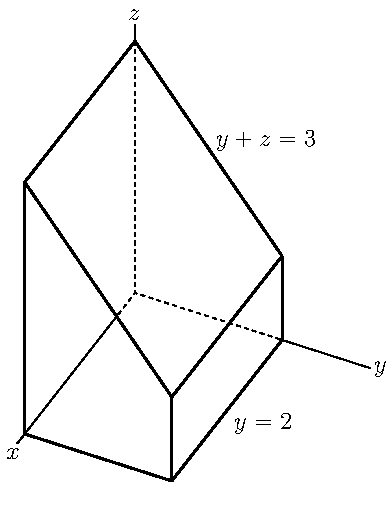
\includegraphics[scale=0.7]{OE16D_8c.pdf}
\end{center}
Now here is the parabolic cylinder $z=x^2$ on the left.
$E$ is constructed by using the parabolic cylinder $z=x^2$ to chop the front
off of the tunnel $x\ge 0$, $0\le y\le 2$, $z\ge 0$,  $y+z\le 3$. The figure 
on the right is a sketch.
\begin{center}
     \includegraphics{OE16D_8d.pdf}\qquad
     \includegraphics{OE16D_8e.pdf}
\end{center}
So
\begin{equation*}
E=\Set{(x,y,z)}{0\le y\le 2,\ x^2\le z\le 3-y}
\end{equation*}

(a) On $E$
\begin{itemize}
\item 
$y$ runs from $0$ to $2$.
\item
For each fixed $y$ in that range, $(x,z)$ runs over
$\Set{(x,z)}{x^2\le z\le 3-y}$.
\item 
In particular, the largest $x^2$ is $3-y$ (when $z=3-y$).
So $x$ runs from $-\sqrt{3-y}$ to $\sqrt{3-y}$.
\item
For fixed $y$ and $x$ as above, $z$ runs from $x^2$ to $3-y$.
\end{itemize}
so that
\begin{align*}
I=\tripInt_E f(x,y,z)\ \dee{V}
= \int_0^2 \int_{-\sqrt{3-y}}^{\sqrt{3-y}} \int_{x^2}^{3-y} f(x,y,z)\ \dee{z}\,\dee{x}\,\dee{y}
\end{align*}

(b) On $E$
\begin{itemize}
\item 
$z$ runs from $0$ to $3$.
\item
For each fixed $z$ in that range, $(x,y)$ runs over
\begin{equation*}
\Set{(x,y)}{0\le y\le 2,\ x^2\le z\le 3-y}
=\Set{(x,y)}{0\le y\le 2,\ y\le 3-z,\ x^2\le z}
\end{equation*}
In particular, $y$ runs from $0$ to the minimum of $2$ and $3-z$.
\item 
So if $0\le z\le 1$ (so that $3-z\ge 2$), 
$(x,y)$ runs over $\Set{(x,y)}{0\le y\le 2,\ x^2\le z}$, while
\item
if $1\le z\le 3$, 
(so that $3-z\le 2$), 
$(x,y)$ runs over $\Set{(x,y)}{0\le y\le 3-z,\ x^2\le z}$,
\end{itemize}
so that
\begin{align*}
I= \int_0^1 \int_0^2 \int_{-\sqrt{z}}^{\sqrt{z}} f(x,y,z)\    
                 \dee{x}\,\dee{y}\,\dee{z}
+\int_1^3 \int_0^{3-z} \int_{-\sqrt{z}}^{\sqrt{z}} f(x,y,z)\    
                 \dee{x}\,\dee{y}\,\dee{z}
\end{align*}

(c) On $E$
\begin{itemize}
\item 
$z$ runs from $0$ to $3$.
\item
For each fixed $z$ in that range, $(x,y)$ runs over
\begin{equation*}
\Set{(x,y)}{0\le y\le 2,\ x^2\le z\le 3-y}
\end{equation*}
In particular, $y$ runs from $0$ to the minimum of $2$ and $3-z$.
\item 
So if $0\le z\le 1$ (so that $3-z\ge 2$), 
$(x,y)$ runs over $\Set{(x,y)}{0\le y\le 2,\ x^2\le z}$, while
\item
if $1\le z\le 3$, 
(so that $3-z\le 2$), 
$(x,y)$ runs over $\Set{(x,y)}{0\le y\le 3-z,\ x^2\le z}$,
\end{itemize}
so that
\begin{align*}
I= \int_0^1  \int_{-\sqrt{z}}^{\sqrt{z}}\int_0^2 f(x,y,z)\    
                 \dee{y}\,\dee{x}\,\dee{z}
+\int_1^3 \int_{-\sqrt{z}}^{\sqrt{z}}  \int_0^{3-z} f(x,y,z)\    
                 \dee{y}\,\dee{x}\,\dee{z}
\end{align*}
\end{solution}

%%%%%%%%%%%%%%%%%%%%%%%%%%%%%%%%
\begin{question}[M200 2002D] %8
Evaluate $\tripInt_E z\,\dee{V}$, where $E$ is the region bounded
by the planes $y=0$, $z=0$ $x+y=2$ and the cylinder $y^2+z^2=1$ in the
first octant.
\end{question}

\begin{hint}
Sketch $E$. You can picture $E$ by thinking of the region bounded by the
planes $x=0$, $y=0$, $z=0$ and $x+y=2$ as a large wedge of cheese and thinking
of the cylinder $y^2+z^2=1$ as a drill hole in the wedge. Then to set up
the limits of integration, first sketch a top view of $E$.
\end{hint}

\begin{answer}
$\frac{13}{24}\approx 0.5417$
\end{answer}

\begin{solution}
The cylinder $y^2+z^2=1$ is centred on the $x$ axis. The part of the cylinder
in the first octant intersects the plane $z=0$ in the line $y= 1$,
intersects to plane $y=0$ in the line $z=1$ and intersects the plane
$x=0$ in the quarter circle $y^2+z^2=1$, $x=0$, $y,z\ge 0$. Here is a
sketch of $E$.
\begin{center}
     \includegraphics{OE02DQ8b.pdf}
\end{center}
Viewed from above, the region
$E$ is bounded by the lines $x=0$, $y=0$, $x+y=2$ and $y=1$. This base region
is pictured below.
\begin{center}
     \includegraphics{OE02DQ8.pdf}
\end{center}
To set up the domain of integration, let's decompose the base region into
horizontal strips as in the figure above. On the base region
\begin{itemize}
\item 
   $y$ runs from $0$ to $1$ and
\item 
   for each fixed $y$ between $0$ and $1$, $x$ runs from $0$ to $2-y$.
\item
   For each fixed $(x,y)$ in the base region $z$ runs from $0$ 
   to $\sqrt{1-y^2}$
\end{itemize}
So
\begin{equation*}
E=\Set{(x,y,z)}{0\le y\le 1,\ 0\le x\le 2-y,\ 0\le z\le\sqrt{1-y^2} }
\end{equation*}
and
\begin{align*}
\tripInt_E z\,\dee{V}&=\int_0^1 \dee{y}\int_0^{2-y}\dee{x}\int_0^{\sqrt{1-y^2}}\dee{z}\ z\\
&=\int_0^1 \dee{y}\int_0^{2-y}\dee{x}\ \frac{1}{2} z^2\Big|_0^{\sqrt{1-y^2}} \\
&=\int_0^1 \dee{y}\int_0^{2-y}\dee{x}\ \frac{1}{2} (1-y^2) \\
&=\int_0^1 \dee{y}\ \frac{1}{2} (1-y^2)(2-y)
=\frac{1}{2}\int_0^1 \dee{y}\ \big(2-y-2y^2+y^3\big) \\
&=\frac{1}{2}\left[2-\frac{1}{2}-\frac{2}{3}+\frac{1}{4}\right]
=\frac{13}{24}\approx 0.5417
\end{align*}
\end{solution}

%%%%%%%%%%%%%%%%%%%%%%%%%%%%%%%%%%%%%%%%%
\begin{question} [M200 2001D] % 8
Find $\dst\tripInt_D x\,\dee{V}$ where $D$ is the tetrahedron bounded
by the planes $x=1$, $y=1$, $z=1$, and $x+y+z=2$.
\end{question}

%\begin{hint}
%
%\end{hint}

\begin{answer}
$\frac{1}{8}=0.125$
\end{answer}

\begin{solution}
The planes $x=1$, $y=1$, $z=1$, and $x+y+z=2$ and the region $D$ are 
sketched below.
\begin{center}
     \includegraphics{OE01DQ8b.pdf}
\end{center}
And here is a sketch of $D$ without the planes cluttering up the figure.
\begin{center}
     \includegraphics{OE01DQ8c.pdf}
\end{center}
On $D$
\begin{itemize}
\item
$z$ runs from $0$ to $1$ and
\item
for each fixed $z$, between 0 and 1, $(x,y)$ runs over the
triangle $T_z$ bounded by $x=1$, $y=1$ and $x+y=2-z$. Observe that when $z=0$,
this triangle is just a point (the bottom vertex of the tetrahedron). 
As $z$ increases, the triangle grows, reaching its maximum size when $z=1$.
\end{itemize}
Here is a sketch of $T_z$.
\begin{center}
     \includegraphics{OE01DQ8.pdf}
\end{center}
In setting up the domain of integration, we'll decompose, for each 
$0\le z\le   1$, $T_z$ into vertical strips as in the figure above.
On $T_z$
\begin{itemize}
\item
$x$ runs from $1-z$ to $1$ and
\item
for each fixed $x$ between $1-z$ and $1$, $y$ runs from $2-x-z$ to $1$
\end{itemize}
so that
\begin{align*}
\tripInt_D x\,\dee{V}
&=\int_0^1\dee{z}\dblInt_{T_z}\dee{x}\,\dee{y}\ x
=\int_0^1 \dee{z}\int_{1-z}^1 \dee{x}\int_{2-x-z}^1 \dee{y}\ x \\
&=\int_0^1 \dee{z}\int_{1-z}^1 \dee{x}\ x(x+z-1)\\
&=\int_0^1 \dee{z}\ \left[\frac{1}{3}x^3+\frac{1}{2} x^2(z-1)\right]_{1-z}^1\\
&=\int_0^1 \dee{z}\ \left[\frac{1}{3}+\frac{1}{2} (z-1)-\frac{1}{3}(1-z)^3
-\frac{1}{2}(1-z)^2(z-1)\right]\\
&=\int_0^1 \dee{z}\ \left[\frac{1}{3}+\frac{1}{2} (z-1)
                               -\frac{1}{6}(z-1)^3\right]\\
&=\left[\frac{1}{3}z+\frac{1}{4} (z-1)^2-\frac{1}{24}(z-1)^4\right]_0^1
=\frac{1}{3}-\frac{1}{4}+\frac{1}{24}=\frac{3}{24} \\
&=\frac{1}{8}=0.125
\end{align*}
\end{solution}

\goodbreak
%%%%%%%%%%%%%%%%%%%%%%%%%%%%%%%%%%%%%%%%%
\begin{question} [M200 2001A] % 8
The solid region $T$ is bounded by the planes $x=0$, $y=0$, 
$z=0$, and $x+y+z=2$ and the surface $x^2+z=1$.
\begin{enumerate}[(a)]
\item
Draw the region indicating coordinates of all corners.

\item
Calculate $\tripInt_T x\,\dee{V}$.
\end{enumerate}
\end{question}

%\begin{hint}
%
%\end{hint}

\begin{answer}
(a)
Here is a 3d sketch of the region. The coordinates of the labelled corners are
\begin{equation*}
a=(0,0,1)\quad
b=(0,0,0)\quad
c=(1,0,0)\quad
d=(0,1,1)\quad
f=(0,2,0)\quad
g=(1,1,0)
\end{equation*}
\begin{center}
     \includegraphics{OE01AQ8b.pdf}
\end{center}


(b) $\frac{17}{60}$
\end{answer}

\begin{solution}
(a)
Here is a 3d sketch of the region. The coordinates of the labelled corners are
\begin{equation*}
a=(0,0,1)\quad
b=(0,0,0)\quad
c=(1,0,0)\quad
d=(0,1,1)\quad
f=(0,2,0)\quad
g=(1,1,0)
\end{equation*}
\begin{center}
     \includegraphics{OE01AQ8b.pdf}
\end{center}

(b) Here is a sketch of the side view of $T$, looking down the $y$ axis. 
\begin{center}
     \includegraphics{OE01AQ8a.pdf}
\end{center}
We'll set up the limits of integration by using it as the base region.
We decompose the base region into vertical strips as in the figure above.
On the base region
\begin{itemize}
\item
$x$ runs from $0$ to $1$ and
\item 
for each fixed $x$ between $0$ and $1$, $z$ runs from $0$ to $1-x^2$.
\item
In $T$, for each fixed $(x,y)$ in the base region, $y$ runs from $0$ to
$2-x-z$.
\end{itemize}
So
\begin{align*}
\tripInt_T x\,\dee{V}
&=\int_0^1\dee{x}\int_0^{1-x^2}\dee{z}\int_0^{2-x-z}\dee{y}\ x
=\int_0^1\dee{x}\int_0^{1-x^2}\dee{z}\ (2-x-z)x\cr
&=\int_0^1 \dee{x}\ \left[x(2-x)(1-x^2)-\frac{1}{2} x{(1-x^2)}^2\right] \\
&=\int_0^1 \dee{x}\ \left[2x-x^2-2x^3+x^4-\frac{1}{2} x+x^3
             -\frac{1}{2} x^5\right] \\
&=\int_0^1 \dee{x}\ \left[\frac{3}{2}x-x^2-x^3+x^4-\frac{1}{2} x^5\right] \\
&=\left[\frac{3}{4}x^2-\frac{1}{3}x^3-\frac{1}{4}x^4+\frac{1}{5}x^5 -\frac{1}{12}x^6\right]_0^1 \\
&=\frac{3}{4}-\frac{1}{3}-\frac{1}{4}+\frac{1}{5}-\frac{1}{12}
=\frac{17}{60}
\end{align*}
\end{solution}



%%%%%%%%%%%%%%%%%%
%\subsection*{\Application}
%%%%%%%%%%%%%%%%%%
